\documentclass{article}
\usepackage{style_sos}
\usepackage{amsmath, amssymb, amsfonts, amsthm, mathtools}
\usepackage[utf8]{inputenc}
\usepackage[inline]{enumitem}
\usepackage{physics}
\usepackage{cancel}
\usepackage{soul}
\usepackage{hyperref}
\hypersetup{
    colorlinks=true,
    linkcolor=black,
    urlcolor=blue,
}
\usepackage{tikz-cd}
\usepackage{tikz}
\usetikzlibrary{decorations.markings, decorations}
\usetikzlibrary{arrows, positioning}
\usepackage{changepage}
\usepackage{subcaption}
\usepackage[section]{placeins}
\usepackage{lipsum, caption, graphicx, nicefrac}
\usepackage{float}
\usepackage{commath}
\usepackage[nottoc,notlot,notlof]{tocbibind}
\usepackage{adjustbox}
\usepackage{color}
\usepackage{tfrupee}
\usepackage{colortbl}
\restylefloat{figure}
\newcolumntype{P}[1]{>{\centering\arraybackslash}p{#1}}
\colorlet{shade}{gray!40}

\theoremstyle{definition}
\newtheorem{theorem}{Theorem}[section]
\newtheorem{lem}[theorem]{Lemma}
\newtheorem{cor}[theorem]{Corollary}
\newtheorem{defn}[theorem]{Definition}
\newtheorem{prop}{Proposition}
\newtheorem{ax}{Axiom}


\setlength\parindent{0pt}
\let\emptyset\varnothing

\newcommand{\Int}{\operatorname{Int}}
\newcommand\ddfrac[2]{\frac{\displaystyle #1}{\displaystyle #2}}
\newlist{steps}{enumerate}{1}
\setlist[steps, 1]{label = Step \arabic*:}
\newenvironment{claim}[1]{\par\noindent\underline{Claim:}\space#1}{}
\setcounter{tocdepth}{1}


\title{Game Theory}
\author{
  Ishan Kapnadak\\
  190070028\\
  Undergraduate, Department of Electrical Engineering\\
  Indian Institute of Technology, Bombay\\
  Summer of Science, 2020\\
  Mentor : Anjali Yadav
}
\smallauthor{Ishan Kapnadak}
\begin{document}

\maketitle
\begin{adjustwidth}{10mm}{10mm}
	\begin{abstract}
	\centering
	This is a short report exploring a wide variety of concepts and applications of Game Theory. We begin with a theoretical framework, exploring various ideas and concepts in Game Theory. We then consider a plethora of interesting real-life scenarios. Finally, we consider the applications of Game Theory in many fields, namely - Quantum Game Theory, Evolutionary Game Theory, Voting Mechanisms, Auctions, Epidemics and Optimal Allocations.
	\end{abstract}
\end{adjustwidth}
\tableofcontents
\bigskip

\addcontentsline{toc}{section}{\textbf{The Theoretical Framework}}

\section{Introduction and Definitions}

\subsection{What is a Game?} 

Game Theory is a branch of mathematics that studies strategic and \textit{interdependent} interaction between two or more people/entities. In simple words, interdependence means that what I do affects you and what you do affects me. An interdependent scenario is one where everyone is affected by each others decisions. While the word ``game'' is most commonly used in the video-game sense, a game is a much broader term in Game Theory. A \textbf{game} is a situation where two or more people are making decisions and these decisions affect all the decision-makers. \medskip

Essentially, Game Theory is a mathematical model analysing situations where multiple players are all striving to satisfy their own interests. Game Theory hinges on the assumption that every player is a \textbf{rational, intelligent} decision-maker. A rational decision-maker is one who always takes decisions or ``plays'' in a way which maximises his/her own `profit'. In other words, a rational player is one who makes decisions in a way to maximise some notion of a profit or a reward. This profit is called the payoff or utility of that player. An intelligent player on the other hand, is one who has the ability to compute best strategies to maximise his/her payoff. 

\subsection{Terminologies}

Before we start analysing games, we will lay down some definitions and terminologies.

\begin{defn}
\textit{Players:} These are the decision-makers in the context of a game. 
\end{defn}
\begin{defn}
\textit{Actions:} These are the list of decisions available to the players. They tell us what the players can do.
\end{defn}
\begin{defn}
\textit{Payoffs:} These are the entities which represent the motivations of our players. Players try to maximise their payoffs during the course of a game.
\end{defn}
\begin{defn}
\textit{Game:} As stated earlier, a game is a scenario or a circumstance where the result of every player is dependent on the decisions of all the players.
\end{defn}
\begin{defn}
\textit{Utility Functions:} These are a set of rules mapping collective strategies of players to their corresponding payoffs. Basically, this tells us how much each player ``earns'' given the decisions made by each player.
\end{defn}
\begin{defn}
\textit{Common Knowledge:} A fact is common knowledge if every player knows it, and every player knows that every player knows it and so on. 
\end{defn}
\begin{defn}
    \textit{Zero-Sum Game:} A game where one player's loss is the other's gain. A zero-sum game is one where the sum of utilities of all the players is zero in \textit{every} outcome.
\end{defn}

\subsection{Representation of Games}

There are two forms of representation. Namely, 

\begin{enumerate}
    \item Normal Form (or Strategic Form)
    \item Extensive Form
\end{enumerate}

First, let us look at the Normal Form of a game. \medskip

A normal form game is basically a \textit{tuple}. It lists the payoffs as a function of actions/decisions taken by the players. Mathematically, we represent the normal form of a game as the tuple 

\[
    \Gamma_{\text{strategic}} = \langle N, (S_i)_{i \in N}, (u_i)_{i \in N} \rangle \quad \text{or} \quad \Gamma_{\text{strategic}} = \langle N, S, u \rangle
\]
Here, $N = \{1, \ldots, n\}$ is the set of $n$ players, indexed by a variable $i \in N$. $S_i$ is the set of actions or pure strategies for player $i$. A particular scenario in the game is described by the set of strategies decided by each player. This is represented as $s = (s_1, \ldots ,s_n) \in S = S_1 \times \ldots \times S_n$, the \textit{strategy profile}. $u_i$ is the utility function for player $i$, which is a function $u_i : S \rightarrow \mathbb{R}$. The set of all utility functions $u = (u_1, \ldots ,u_n)$ is known as the \textit{utility profile}. \medskip

An Extensive Form of a game, on the other hand, is a representation of games in the form of a \textit{decision tree}. The edges in the tree represent the actions taken by the player. The value of the source node specifies which player takes the action of the corresponding edges. Every branch ends in an outcome, which specifies the payoffs of every player corresponding to that scenario. \medskip

Mathematically, we can represent the extensive form as the tuple:

\[
    \Gamma_{\text{extensive}} = \langle N, (A_i)_{i \in N}, \mathbb{H}, \mathcal{P}, (\mathbb{I}_i)_{i \in N}, (u_i)_{i \in N} \rangle    
\]

Here, $N = \{ 1, \ldots , n \}$ denotes the list of players. $A_i$ denotes the action set of player $i$. $\mathbb{H}$ denotes the set of all terminal histories - namely the set of paths to each terminal. $S_\mathbb{H}$ denotes the set of proper sub-histories of the terminal histories. $\mathcal{P} : S_\mathbb{H} \rightarrow N$ denotes a mapping of all proper sub-histories to the players. $\mathbb{I}_i$ denotes the set of all information sets of player $i$. $u_i : \mathbb{H} \rightarrow \mathbb{R}$ is the utility function of player $i$.

\medskip

\textbf{Example - Rock, Paper and Scissors} \medskip

\begin{figure}[!h]
  \centering
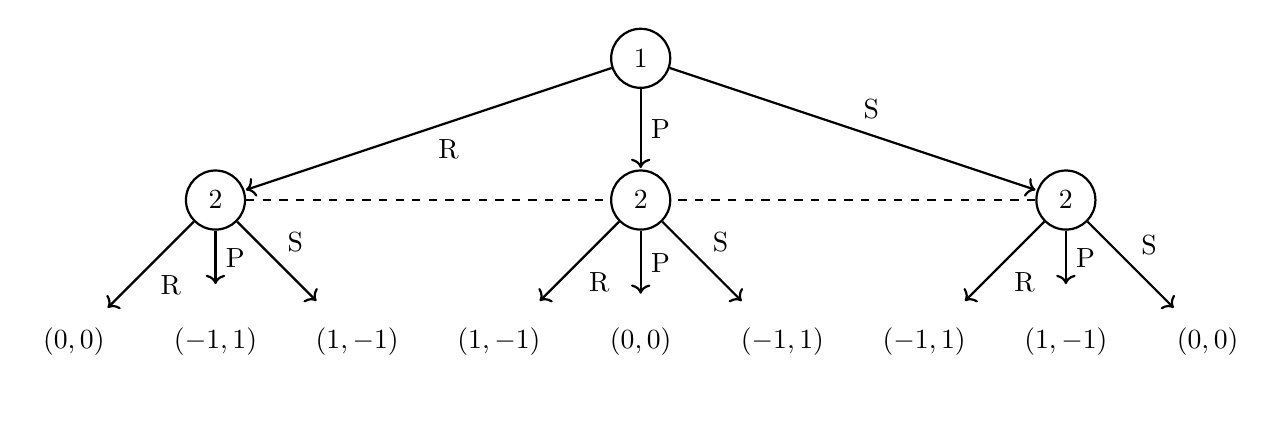
\begin{tikzpicture}[shorten >=0.5pt,node distance=1.8cm,on grid,auto]
    \tikzstyle{state}=[shape=circle,thick,draw,minimum size=0.75cm]
    \tikzstyle{outcome}=[shape=circle, minimum size=0.75cm]

    \node[state] (A1) { $1$};
    
    \node[state,below of=A1] (B1) {$2$};
    \node[outcome, right of=B1] (B_1) {};
    \node[outcome, right of=B_1] (B__1) {};
    \node[state, right of=B__1] (B2) {$2$};
    \node[outcome, left of=B1] (B_0) {};
    \node[outcome, left of=B_0] (B__0) {};
    \node[state, left of=B__0] (B0) {$2$};
    
    \node[outcome,below of=B0] (C1) {$(-1,1)$};
    \node[outcome, right of=C1] (C2) {$(1,-1)$};
    \node[outcome, left of=C1] (C0) {$(0,0)$};
    
    \node[outcome,below of=B1] (C4) {$(0,0)$};
    \node[outcome, right of=C4] (C5) {$(-1,1)$};
    \node[outcome, left of=C4] (C3) {$(1,-1)$};
    
    \node[outcome,below of=B2] (C7) {$(1,-1)$};
    \node[outcome, right of=C7] (C8) {$(0,0)$};
    \node[outcome, left of=C7] (C6) {$(-1,1)$};
    
    \path[->,draw,thick]
    (A1) edge node {R} (B0)
    (A1) edge node {P} (B1)
    (A1) edge node {S} (B2)
    (B0) edge node {R} (C0)
    (B0) edge node {P} (C1)
    (B0) edge node {S} (C2)
    (B1) edge node {R} (C3)
    (B1) edge node {P} (C4)
    (B1) edge node {S} (C5)
    (B2) edge node {R} (C6)
    (B2) edge node {P} (C7)
    (B2) edge node {S} (C8)
    
    ;
    
    \draw[dashed] (B0) -- (B1);
    \draw[dashed] (B2) -- (B1);

  \end{tikzpicture} 
  \caption{Extensive Form of Rock, Paper, Scissors}
  \label{fig:tree1}
\end{figure}

Here, the dotted line connecting the decisions of player $1$ shows that player $2$ has no knowledge about player $1$'s decision beforehand. A set of nodes connected via dotted lines forms an \textbf{information set}. An information set establishes or lists down all the possible moves that could have happened previously. 

For this game, we have:

\begin{itemize}
    \item $N = \{ 1,2 \}$
    \item $S_1 = S_2 = \{\text{Rock, Paper, Scissors} \}$ or more conveniently denoted as $\{ \text{R, P, S}\}$
    \item $\mathbb{H} = \{ (R,R), (R,P), (R,S), (P,R), (P,P), (P,S), (S,R), (S,P), (S,S) \}$
    \item $S_\mathbb{H} = \{ \epsilon , R, P, S\}$. Here, $\epsilon$ denotes the empty history. 
    \item $\mathcal{P}(\epsilon) = 1; \quad \mathcal{P}(R) = \mathcal{P}(P) = \mathcal{P}(S) = 2 $
    \item $\mathbb{I}_1 = \{ \{ \epsilon \} \}; \quad \mathbb{I}_2 = \{ \{ R, P, S \} \}$
    \item $u_1(R,R) = 0; \quad u_1(R,P) = -1; \quad u_1(R,S) = 1; \quad u_1(P,R) = 1; \quad u_1(P,P) = 0; \quad u_1(P,S) = -1; \quad u_1(S,R) = -1; \quad u_1(S,P) = 1; \quad u_1(S,S) = 0$
    \item $u_2(R,R) = 0; \quad u_2(R,P) = 1; \quad u_2(R,S) = -1; \quad u_2(P,R) = -1; \quad u_2(P,P) = 0; \quad u_2(P,S) = 1; \quad u_2(S,R) = 1; \quad u_2(S,P) = -1; \quad u_2(S,S) = 0$
\end{itemize}

This same game can also be represented in the normal form. In the normal form, we represent the utility functions as a table known as the \textbf{payoff matrix}. Following is the payoff matrix for a round of rock, paper and scissors. By convention, we shall assume that the moves listed along the rows are the moves of Player $1$ and those listed along the columns are those of Player $2$. \medskip 
\begin{table}[H]
    \begin{adjustbox}{width=8cm,center}
    \begin{tabular}{|c|c|c|c|}
        \hline
        1 \textbackslash \: 2 & Rock & Paper & Scissors \\
        \hline
        Rock & 0,0 & -1,1 & 1,-1 \\
        \hline 
        Paper & 1,-1 & 0,0 & -1,1 \\
        \hline
        Scissors & -1,1 & 1,-1 & 0,0\\
        \hline
    \end{tabular}
    \end{adjustbox}
    \caption{Payoff Matrix for Rock, Paper, Scissors}
    \label{table:rps1}
\end{table}

For this game, we have 

\begin{itemize}
    \item $N = \{1,2\}$
    \item $S_1 = S_2 = \{\text{Rock, Paper, Scissors} \}$ or more conveniently denoted as $\{ \text{R, P, S}\}$
    \item $u_1(R,R) = 0; \quad u_1(R,P) = -1; \quad u_1(R,S) = 1; \quad u_1(P,R) = 1; \quad u_1(P,P) = 0; \quad u_1(P,S) = -1; \quad u_1(S,R) = -1; \quad u_1(S,P) = 1; \quad u_1(S,S) = 0$
    \item $u_2(R,R) = 0; \quad u_2(R,P) = 1; \quad u_2(R,S) = -1; \quad u_2(P,R) = -1; \quad u_2(P,P) = 0; \quad u_2(P,S) = 1; \quad u_2(S,R) = 1; \quad u_2(S,P) = -1; \quad u_2(S,S) = 0$
\end{itemize}

\textbf{Some other notations for Strategic Form Games:}

\begin{enumerate}
        \item The index $-i$ is used to refer to all the players other than player $i$.
        \item $s_{-i}$ is the strategy profile of all players other than player $i$.
        \item The complete strategy profile can further be denoted as $(s_i, s_{-i})$.
\end{enumerate} 

\section{Strict Dominance, Weak Dominance and Equilibria}

\subsection{Introduction and the Prisoner's Dilemma}

\begin{defn}
\textit{Strict Dominance:} A strategy $\mathcal{X}$ is said to strictly dominate a strategy $\mathcal{Y}$ if strategy $\mathcal{X}$ generates a greater payoff than strategy $\mathcal{Y}$ regardless of what other players do. \medskip

Mathematically, given a strategic form game $\Gamma = \langle N, S, u\rangle$, a strategy $s_i \in S_i$ of a player $i$ is said to strictly dominate another strategy $s^{\prime}_i \in S_i$ if 

\[
    u_i(s_i, s_{-i}) > u_i(s^{\prime}_i, s_{-i}) \: \forall \: s_{-i} \in S_{-i}
\]
\end{defn}

\begin{defn}
\textit{Strictly Dominant Strategy Equilibrium:}  Given a strategic form game $\Gamma = \langle N, S, u\rangle$, a strategy profile $s^* = (s^{*}_1, \ldots , s^{*}_n)$ is called a strictly dominant strategy equilibrium if the strategy $s^{*}_i$ is a strictly dominant strategy for every player $i$, i.e, $\forall \: i = 1,2, \ldots n$.
\end{defn}

Consider the payoff matrix for the Prisoner's Dilemma, shown in Table \ref{table:pris_dil1}. There are two prisoners involved in a robbery. Each has the option of defecting on his partner (confess) or staying silent. 

\begin{table}[H]
    \begin{adjustbox}{width=6cm,center}
    \begin{tabular}{|c|c|c|}
        \hline
        A \textbackslash \: B & Silent & Confess \\
        \hline
        Silent & -1,-1 &  -12,0 \\
        \hline 
        Confess & 0,-12 & -8,-8  \\
        \hline
    \end{tabular}
    \end{adjustbox}
    \caption{Payoff Matrix the Prisoner's Dilemma}
    \label{table:pris_dil1}
\end{table}

Confession is a strictly dominant strategy for both suspects and hence, (confess, confess) is a strictly dominant strategy equilibrium. While both keeping quiet is a \textit{mutually} better scenario for each of them, each of them could do \textit{individually} better by confessing. Hence, it is sensible for both of them to confess. \medskip

\begin{defn}
\textit{Weak Dominance:} Given a strategic form game $\Gamma = \langle N, S, u\rangle$, a strategy $s_i \in S_i$ is said to weakly dominate another strategy $s^{\prime}_i \in S_i$ for player $i$ if

\[
    u_i(s_i, s_{-i}) \geq u_i(s^{\prime}_i, s_{-i}) \: \forall \: s_{-i} \in S_{-i} \quad \text{and} \quad u_i(s_i, s_{-i}) > u_i(s^{\prime}_i, s_{-i}) \: \text{for some} \: s_{-i} \in S_{-i}
\]
\end{defn}
\begin{defn}
\textit{Very Weak Dominance:} Given a strategic form game $\Gamma = \langle N, S, u\rangle$, a strategy $s_i \in S_i$ is said to very weakly dominate another strategy $s^{\prime}_i \in S_i$ for player $i$ if

\[
    u_i(s_i, s_{-i}) \geq u_i(s^{\prime}_i, s_{-i}) \: \forall \: s_{-i} \in S_{-i}
\]
\end{defn}
\begin{defn}
\textit{Weakly Dominant Strategy Equilibrium:}  Given a strategic form game $\Gamma = \langle N, S, u \rangle$, a strategy profile $s = (s^{*}_1, \ldots , s^{*}_n)$ is called a weakly dominant strategy equilibrium if the strategy $s^{*}_i$ is a weakly dominant strategy for every player $i$, i.e, $\forall \: i = 1,2, \ldots n$.
\end{defn}
\begin{defn}
\textit{Very Weakly Dominant Strategy Equilibrium:}  Given a strategic form game $\Gamma = \langle N, S, u \rangle$, a strategy profile $s = (s^{*}_1, \ldots , s^{*}_n)$ is called a very weakly dominant strategy equilibrium if the strategy $s^{*}_i$ is a very weakly dominant strategy for every player $i$, i.e, $\forall \: i = 1,2, \ldots n$.
\end{defn}
\begin{defn}
    \textit{Pareto Dominance:} Given a strategic form game $\Gamma = \langle N, S, u \rangle$, we say that a particular outcome $o$ of the game Pareto-dominates another outcome $o^{\prime}$ if both these statements hold:
    \begin{enumerate}
        \item 
            $u_i(o_i) \geq u_i(o^{\prime}) \quad \forall \: i \in N$.
        \item 
            $ u_i(o_i) > u_i(o^{\prime})$ for some $i \in N$.
    \end{enumerate}
\end{defn}

\begin{defn}
    \textit{Pareto Optimality:} An outcome $o^{\prime}$ is Pareto-optimal if there is no outcome which Pareto-dominates it.
\end{defn}

\subsection{Iterated Elimination of Strictly Dominated Strategies}

We shall now discuss a method to solve more complex games than the Prisoner's Dilemma. By ``solving'' a game, we mean applying logical deductions to arrive at the final outcome(s) of the game if it was played by intelligent, rational players. Consider the following \textit{non-symmetric} game. \medskip
\begin{table}[H]
    \begin{adjustbox}{width=6cm,center}
    \begin{tabular}{|c|c|c|c|}
        \hline
        A \textbackslash \: B & Left & Centre & Right \\
        \hline
        Up & 10,3 & 7,3 & 1,4 \\
        \hline 
        Middle & 4,1 & 6,2 & 3,3 \\
        \hline
        Down & -1,9 & 8,-1 & 2,8\\
        \hline
    \end{tabular}
    \end{adjustbox}
    \caption{Payoff Matrix for a certain game}
    \label{table:iesds}
\end{table}

To solve this game, we apply an algorithm known as \textbf{Iterated Elimination of Strictly Dominated Strategies} (IEDS). As the name suggests, on every iteration, we eliminate a strategy which is strictly dominated and solve the simplified game. This is based on the fact that no player would ever play a strictly dominated strategy. Following are the steps to solve this game. 

\begin{steps}
    \item First, observe that `Centre' is a strictly dominated strategy for Player B. For every move that Player A plays, playing `Right' provides greater payoff to Player B than playing `Centre'. Hence, we eliminate the `Centre' column from the game as it is a strictly dominated strategy. The simplified game is now: \medskip
    \begin{table}[H]
    \begin{adjustbox}{width=5cm,height=1.2cm,center}
    \begin{tabular}{|c|c|c|}
        \hline
        A \textbackslash \: B & Left & Right \\
        \hline
        Up & 10,3 & 1,4 \\
        \hline 
        Middle & 4,1 & 3,3 \\
        \hline
        Down & -1,9 & 2,8\\
        \hline
    \end{tabular}
    \end{adjustbox}
    \caption{Payoff Matrix after Step 1}
    \label{table:iesds_step1}
    \end{table}
    
    \item Next, observe that `Down' is a strictly dominated strategy for Player A. The strategy `Middle' always generates a greater payoff than `Down'. Hence, we eliminate the `Down' row. The simplified game is now: \medskip
    \begin{table}[H]
    \begin{adjustbox}{width=5cm,center}
    \begin{tabular}{|c|c|c|}
        \hline
        A \textbackslash \: B & Left & Right \\
        \hline
        Up & 10,3 & 1,4 \\
        \hline 
        Middle & 4,1 & 3,3 \\
        \hline
    \end{tabular}
    \end{adjustbox}
    \caption{Payoff Matrix after Step 2}
    \label{table:iesds_step2}
    \end{table}
    
    \item Now it is easy to see that `Right' is the strictly dominant strategy for Player B, hence he plays `Right'. Player A \textit{knows} that Player B would play `Right', hence he plays `Middle' to maximise his own payoff. Hence, the final outcome is a payoff of $(3,3)$ when Player B plays `Right' and Player A plays `Middle'. 
    
\end{steps}

This end result wasn't an obvious outcome or an easy one to come by. But, we could successively eliminate strictly dominated strategies at every step to simplify the game and arrive at the end result. \medskip

\section{Pure Strategy Nash Equilibria}

\subsection{Introduction and the Stag Hunt}

\begin{defn}
\textit{Pure Strategy Nash Equilibrium:} A pure strategy Nash equilibrium (PSNE) is a set of strategies (one for each player) such that no player can benefit by changing his/her strategy in the given situation. \medskip

Mathematically, given a strategic form game $\Gamma = \langle N, S, u \rangle$, a strategy profile $s = (s^{*}_1, \ldots , s^{*}_n)$ is called a pure strategy Nash equilibrium of $\Gamma$ if
\[
    u_i(s^{*}_i, s^{*}_{-i}) \geq u_i(s_i, s^{*}_{-i}) \: \forall \: s_i \in S_i \quad \text{and} \quad \forall \: i = 1,2,\ldots , n
\]
\end{defn}

While looking for PSNE, we are only interested in \textit{individual or unilateral deviations}. That is, players will maintain their current strategy given that all others maintain the same strategy as well. Nash equilibria are inherently stable. This is because every player is optimally responding to what every other player is doing, hence none of the players regret what they are doing. \medskip

The dominant strategy equilibria, if they exist, are very desirable. However these equilibria are rarely found in the real world. Nash equilibria are more common and are a weaker notion of these equilibria. \medskip

We now discuss another classic Game Theory problem known as the Stag Hunt. Consider that there are two hunters who are going for hunting one day. They can either hunt a stag or a hare. The stag is worth $10$ meat units while the hare is worth $2$ meat units. There are two hares present. To hunt a stag, both the hunters need to combine their efforts. The meat is then shared between both of them. However, a hunter can hunt hares individually. On the day of the hunt, they both must individually decide which equipment to carry along with them - one to hunt stags or one to hunt hares. If both are hunting stags, then both of them share the stag meat. If one of them hunts for stags while the other doesn't, then the hare hunter gets both the hares while the stag hunter gets nothing. If both of them hunt hares then each gets one hare. They want to maximise the amount of meat they take on the day of the hunt. We can represent this situation as the following payoff matrix. \medskip

\begin{table}[H]
    \begin{adjustbox}{width=5cm,center}
    \begin{tabular}{|c|c|c|}
        \hline
        A \textbackslash \: B & Stag & Hare \\
        \hline
        Stag & \cellcolor{yellow} 5,5 &  0,4 \\
        \hline 
        Hare & 4,0 & \cellcolor{yellow} 2,2  \\
        \hline
    \end{tabular}
    \end{adjustbox}
    \caption{Payoff Matrix for the Stag Hunt. The coloured cells are PSNE}
    \label{table:stag}
\end{table}

In this game, the stag-stag outcome is a PSNE. The hare-hare outcome is also a PSNE, which is a mutually worse outcome for both but it is stable to unilateral deviations. This equilibrium arises because there is no coordination between the hunters. 

Intuitively, a Nash equilibrium is a law people would want to obey even if they could break rules. Consider for example - Traffic signals. \medskip

\textbf{Example.} Consider the scenario where two cars approach each other from perpendicular directions. The traffic signal is green for one and red for the other. The cars could either both go, leading to a crash (payoff: $-10$), or both stop leading to both of them unnecessarily waiting (payoff: $-1$). One of them could go while the other stops leading to payoff $1$ for the person who goes and zero for the one who stops. We analyse the Nash equilibria of the corresponding payoff matrix. \medskip
\begin{table}[H]
    \begin{adjustbox}{width=5cm,center}
    \begin{tabular}{|c|c|c|}
        \hline
        A \textbackslash \: B & Go & Stop \\
        \hline
        Go & -10,-10 &  \cellcolor{yellow} 2,0 \\
        \hline 
        Stop & \cellcolor{yellow} 0,2 & -1,-1  \\
        \hline
    \end{tabular}
    \end{adjustbox}
    \caption{Payoff Matrix for the Traffic Signal Scenario. The coloured cells are PSNE}
    \label{table:traffic}
\end{table}

The coloured scenarios (namely go-stop and stop-go) are the Nash equilibria of this game. The traffic law tells one of the players to go while the other to stop. Hence, it is a law which both cars are following \textit{willingly} as it helps their own self interest. 

\subsection{Best Responses}

\begin{defn}
\textit{Best Response:} Given what all the other players are doing, a strategy is called a best response if and only if the player cannot gain more by switching to a different strategy. \medskip

Mathematically, given a strategic form game $\Gamma = \langle N, S, u \rangle$ and a strategy profile $s_{-i} \in S_{-i}$, we say that a strategy $s_i \in S_i$ is a best response of player $i$ with respect to the profile $s_{-i}$ if $u_i(s_i, s_{-i}) \geq u_i(s^{\prime}_{i}, s_{-i}) \: \forall \: s^{\prime}_{i} \in S_i$.
\end{defn}

Having defined best response this way, we can redefine Nash equilibrium as follows:

\begin{defn}
A game is in Nash Equilibrium if and only if all players are playing their best responses to what other players are playing.
\end{defn}

\subsection{Interpretation of Nash Equilibrium}

Nash equilibrium is a powerful tool in Game Theory. We could think of it as a \textit{prescription}. An adviser would advise his clients to play Nash equilibrium strategy profiles as neither player would want to deviate from this strategy profile if others are following it. This also gives it us the notion of Nash equilibrium being a `\textit{self enforced}' agreement. This is because neither player would want to break the agreement if the other isn't doing so. Note: Nash equilibria talk only about unilateral deviations. It is possible that two players deviate simultaneously, resulting in higher profits for both. For example, in the Prisoner's Dilemma, the confess-confess is a Nash equilibrium. However, both of them could deviate, earning a higher utility. The silent-silent outcome is \textbf{not} a Nash equilibrium, but yet provides better utility for both players. Thus, Nash equilibria \textbf{need not} guarantee maximal utility. They only guarantee maximal utility if everyone else plays the same way. \medskip

Nash equilibrium can also be correlated to dynamic and steady-state phases of adjustment processes. Nash equilibria are usually the points of convergence of such processes. Hence, they can also be thought of as a \textit{prediction} of the most probable outcome. \medskip

It is also important to note that pure strategy Nash equilibria may not exist in all games. For example, Rock, Paper and Scissors does not have a pure strategy Nash equilibrium.

\subsection{Schelling Point}

In games having multiple Nash equilibria, the obvious question to ask is - which of these Nash equilibria would ultimately be implemented? This question was answered via a concept proposed by Thomas Schelling. He says that if something makes every player to focus their attention on a particular equilibrium, then all of them would expect this equilibrium to be implemented and would act accordingly. Such an equilibrium, which has some characteristic that distinguishes it from other equilibria is called a \textbf{Schelling Point} or a \textbf{Focal Point}.

\section{Backward Induction}

Backward Induction is a useful solution concept to solve extensive form games. In this method, we reason backwards from the end of the game to the beginning. It is best to demonstrate this with the help of one of the most interesting riddles I have come across. \medskip

Consider that you are the leader of a (intelligent and rational) pirate group consisting of five members, including you. The pirates are A(you), B,C,D,E. You have just found $100$ coins worth of treasure and it is now time to distribute this treasure amongst you and your co-pirates. The terms of the distribution are as follows:
\begin{enumerate}
    \item You get to propose the first method of distribution. If at least three of the five pirates agree with you, then the distribution stands.
    \item If less than three pirates agree with your distribution, then you are killed and the next pirate (B) gets to propose the distribution. 
    \item If two of the remaining four agree with B's proposition, then it stands otherwise he is killed and C decides the proposition.
    \item This continues iteratively.
\end{enumerate}

Your aim is to maximise the number of coins you get while still being alive. What distribution do you propose? \bigskip

At this point, it is fairly difficult to find a distribution that will maximise your gain yet keeping you alive. But let us start from the end. 

\begin{enumerate}
    \item Consider the scenario where only D and E are left. Any of D's propositions will hold as he needs only one `yes' vote which he can give himself. Thus, he would propose the distribution where he gets all of the $100$ coins and gives none to E. E doesn't want this, but has no say.
    \item C exploits this scenario to his own advantage. C proposes the distribution $(99, 0 , 1)$. By giving a single coin to E, C has guaranteed E's support. This is because if E rejects this proposition, it would lead him back to the above scenario, where he gets nothing. As getting a single coin is better than nothing, both C and E accept this proposition, leaving D with nothing. C doesn't need to give any more than a single coin because even a single coin guarantees E's support. As C wants to maximise his own profit as well, he gives E only one coin.
    \item B exploits this scenario to gain D's vote. He proposes the distribution $(99, 0 , 1 , 0)$. By giving a single coin to D, B has guaranteed D's support. This is because if D rejects this proposition, it would lead him back to the above scenario, where he gets nothing. As getting a single coin is better than nothing, both D and B accept this proposition, which is enough support. This leaves C and E with nothing. 
    \item Finally, you would exploit this scenario to gain C and E's support. You propose the distribution $(98, 0 , 1, 0 ,1)$. By giving a single coin to C and E, you have guaranteed their support as neither of them wants to go to the above scenario where they get nothing. As you have 3 `yes' votes, the distribution stands and you get $98$ out of the $100$ coins !
\end{enumerate}

\section{Mixed Strategies and the Nash Theorem}

\subsection{What are Mixed Strategies?}

The games we have considered so far employ only what are known as pure strategies. A pure strategy is an unconditional, defined choice that a player makes. But of course, this is not a good way to model humans. If I play Rock, Paper and Scissors with someone, I wouldn't want to play the same move over and over again. Instead, I would want to vary my strategies. A mixed strategy provides a natural abstraction of pure strategies that mimic real life strategic behaviour. A mixed strategy is basically a probability distribution over all strategies in the pure strategy set. They concisely represent what would happen if games were played repeatedly. They also describe \textit{population dynamics.} If for a particular game, we have a population of one million Player A's and one million Player B's, and each pair plays the game separately, then we could describe the count of pure strategies obtained neatly via a single mixed strategy.

\begin{defn}
    \textit{Mixed Strategy:} Given a player $i$ having a set $S_i$ of pure strategies, a mixed strategy (or randomized strategy) $\sigma_i$ of that player is a probability distribution. In other words, $\sigma_i : S_i \mapsto [0,1]$ is a mapping that assigns each strategy a probability $\sigma_i(s_i)$ subject to the condition:
    \[
        \sum_{s_i \in S_i} \sigma_i(s_i) = 1
    \]
\end{defn}

\begin{defn}
    \textit{Mixed Strategy Nash Equilibrium:} Given a strategic form game $\Gamma = \langle N, S, u \rangle$, a mixed strategy profile $(\sigma^{*}_1, \ldots , \sigma^{*}_n)$ is a mixed strategy Nash equilibrium if for all $i \in N$
    \[
        u_i(\sigma^{*}_i , \sigma^{*}_{-i}) \geq u_i(\sigma_i, \sigma^{*}_{-i}) \: \forall \: \sigma_i \in \Delta(S_i)
    \]
\end{defn}

\subsection{Battle of the Sexes}

The Battle of the Sexes game is a commonly discussed two-player coordination game (sometimes also referred to as the Bach or Stravinsky game). The scenario is such: Imagine a couple were to meet this evening. But, neither of them can recall where they were supposed to meet - at the opera or the football game. The fact that neither of them can recall is common knowledge. The man (M) is more interested in football, while the woman (W) is more interested in the opera. However, both of them want to be together. If they show up at different places, then both would be sad and go home. Following is the payoff matrix for the scenario: \medskip

\begin{table}[H]
    \begin{adjustbox}{width=5cm,center}
    \begin{tabular}{|c|c|c|}
        \hline
        M \textbackslash \: W & Football & Opera \\
        \hline
        Football & 2,1 & 0,0 \\
        \hline 
        Opera & 0,0 & 1,2  \\
        \hline
    \end{tabular}
    \end{adjustbox}
    \caption{Payoff Matrix for the Battle of the Sexes}
    \label{table:bos}
\end{table}

Let us find a mixed strategy equilibrium for this game. Consider that the man allots a probability of $\sigma_M$ to football and that the woman allots a probability of $\sigma_W$ to football. For this to be a mixed strategy equilibrium, each player must be indifferent about his/her choices given the other players' strategies. Hence, we equate the expected payoffs for both strategies and for both players. This gives us the following two equations 
\[
    \sigma_W \cdot 2 + (1-\sigma_W) \cdot 0 = \sigma_W \cdot 0 +  (1-\sigma_W) \cdot 1
\]
\[
    \sigma_M \cdot 0 + (1- \sigma_M) \cdot 2 = \sigma_M \cdot 1 +  (1-\sigma_M) \cdot 0
\]
On solving, we get $\sigma_M = \frac{2}{3}$ and $\sigma_W = \frac{1}{3}$. Hence, the man going to the football game with probability two-thirds and the woman going to the opera with probability two-thirds is a mixed strategy equilibrium. 

\subsection{The Nash Theorem}

Now that we have covered both pure strategies and mixed strategies, we state perhaps the most important theorem in Game Theory 

\begin{theorem}
\textit{Nash Theorem.} Every finite strategic form game has a Nash equilibrium, either in the pure strategies or in the mixed strategies.
\end{theorem}

A proof of this theorem is way beyond the scope of this report. However, this \href{http://math.uchicago.edu/~may/REU2017/REUPapers/Yuan.pdf}{document} by Allen Yuan proves and explains the Nash theorem in depth.

\subsection{Correlated Equilibria}

Consider the Battle of the Sexes example above. Intuitively, the best outcome would be a $50-50$ split between the outcomes $(F,F)$ and $(O,O)$. But there is no way to perfectly achieve this. If the players play pure strategies, then one of them misses out (say, the man misses out on the $(F,F)$ outcome if the $(O,O)$ is chosen). If they mix up their strategies, it is possible that they will miscoordinate, leading to the unfavourable outcomes $(O,F)$ or $(F,O)$. \smallskip

A similar situation arose in the traffic example, with the (Stop,Go) and (Go,Stop) outcomes. Here, however, there was a traffic signal which indicated one player to take a particular action. A traffic signal behaves as a fair randomizing device which tells each player what action to take randomly. Because of the traffic signal, randomness (and thus, fairness) has been achieved and the negative outcomes are ruled out. We can introduce a similar device to the Battle of the Sexes game, which tells each one of them what to do. This is the idea of a \textbf{Correlated Equilibrium.} \smallskip

A correlated equilibrium is a randomized assignment of actions to players such that neither player would want to deviate. If these actions are not correlated, this leads us back to Nash equilibrium. \smallskip

\textbf{Example.} Consider the chicken game - where two players each have two options, whether to dare (D) or chicken out (C). The payoff matrix for this game is as shown: \medskip

\begin{table}[H]
    \begin{adjustbox}{width=5cm,center}
    \begin{tabular}{|c|c|c|}
        \hline
        1 \textbackslash \: 2 & Dare & Chicken-out \\
        \hline
        Dare & 0,0 & 7,2 \\
        \hline 
        Chicken-out & 2,7 & 6,6  \\
        \hline
    \end{tabular}
    \end{adjustbox}
    \caption{Payoff Matrix for the Chicken Game}
    \label{table:chicken}
\end{table}

A mixed strategy Nash equilibrium for the above scenario has each player daring with a probability of $\frac{1}{3}$. The expected reward for each player can be calculated as:
\[
    u_{\text{avg}} = \frac{1}{3} \cdot \frac{1}{3} \cdot 0 + \frac{1}{3} \cdot \frac{2}{3} \cdot 7 + \frac{2}{3} \cdot \frac{1}{3} \cdot 2 + \frac{2}{3} \cdot \frac{2}{3} \cdot 6 = \frac{42}{9} = 4 \frac{2}{3}
\]
 
Consider now that a trusted party shuffles between the outcomes (C,C), (D,C) and (C,D) with equal probability of $\frac{1}{3}$. If the trusted party tells player $1$ to dare, then he would have no intention of deviating. This is because he knows the outcome would've been (D,C) and player $2$ wouldn't deviate from his strategy either. Hence, this is a correlated equilibrium. The expected award for this equilibrium would be:
\[
    u_{\text{avg}} = \frac{1}{3} \cdot \left( 2 + 7 + 6 \right) = 5
\]

which is greater then the reward for the mixed strategy Nash equilibrium. In a sense, the introduction of a trusted party eliminates any chance of miscoordination and hence increases the overall reward. 

\section{Utility Theory}

So far, we have randomly assigned utility values to outcomes. But how do know that these values accurately represent the preferences of the players? This was answered by the utility theory - developed by John von Neumann and Oskar Morgenstern. \medskip

Suppose a player prefers outcome $a$ to $b$, $b$ to $c$ and $c$ to $d$. We use a binary relation (called a preference relation) to depict this preference order. This is denoted as $a \succ b \succ c \succ d$. However, the preference relation does not tell us what numbers to assign to each outcome. Hence, we can choose any numbers as long as the preference order is maintained. This is known as an ordinal utility function. \medskip

When there is an uncertainty about which outcome will be selected, we use \textit{lotteries} to describe preferences. Suppose $X$ is the outcome set $\{ x_1, x_2, \ldots , x_m \}$, then a lottery on $X$ is a probability distribution:
\[
    \sigma = [ p_1 : x_1; \: p_2 : x_2; \: \ldots \: p_m : x_m ]
    \]
    \[
    p_j \geq 0 \quad \text{for} \: j = 1,2 \ldots , m \quad \text{and} \quad \sum_{j=1}^{m} p_j = 1
\]

Consider that in the above example, we define two lotteries as: $\sigma_1 = [0.3 : a; \: 0.2 : b; \: 0.2 : c; \: 0.3 : d]$ and $\sigma_1 = [0.4 : a; \: 0.15 : b; \: 0.25 : c; \: 0.2 : d]$. The set of all lotteries is denoted by $\Delta(X)$. The question is: which of the two lotteries is preferred by the two players? Note that now the answer depends on the values we assign to each outcome. Hence, we cannot use ordinal utilities anymore. This problem was solved by von Neumann and Morgenstern. \medskip

\subsection{Axioms of von Neumann and Morgenstern}

Consider $X$ to be the set of outcomes. The preferences of player $i$ for the outcomes in $X$ can be represented by a binary relation  $\succsim$ on $X$. Given $x_1, x_2 \in X$, we define the following:

\begin{itemize}
    \item $x_1 \succsim x_2$ : outcome $x_1$ is weakly preferred to outcome $x_2$.
    \item $x_1 \succ x_2$ : outcome $x_1$ is strictly preferred to outcome $x_2$.
    \item $x_1 \sim x_2$ : outcomes $x_1$ and $x_2$ are equally preferred (indifference)
\end{itemize}

Clearly, we have :
\begin{itemize}
    \item $x_1 \succ x_2 \iff x_1 \succsim x_2$ and $\neg{(x_2 \succsim x_1)}$
    \item $x_1 \sim x_2 \iff x_1 \succsim x_2$ and $x_2 \succsim x_1$
\end{itemize}

Note that the preference relation $\succsim$ is a \textit{reflexive} relation and $x \sim x$. We will now state the von Neumann - Morgenstern axioms. These axioms represent naturally arising properties or desirable properties in preferences.

\begin{ax}
\textbf{(Completeness)} \smallskip

The completeness property implies that every possible pair of outcomes in $X$ is related by the preference relation. The preference relation $\succsim$ also induces an ordering over $X$. Formally, 
\[
    x_1 \succ x_2; \; \text{or} \; x_2 \succ x_1; \; \text{or} \; x_1 \sim x_2 \quad \forall \: x_1, x_2 \in X
\]
\end{ax}

\begin{ax}
\textbf{(Transitivity)} \smallskip

The axiom of transitivity states that:
\[
    x_1 \succsim x_2 \; \text{and} \; x_2 \succsim x_3 \implies x_1 \succsim x_3 \: \forall \: x_1, x_2, x_3 \in X
\]
This is a natural requirement. Suppose a player prefers one outcome to another and that to a third, the player would also prefer the first outcome to the third. To support this argument, suppose we had $x_1 \succsim x_2$ and $x_2 \succsim x_3$ but $x_3 \succ x_1$. If the player started out with outcome $x_1$, he would want to trade it for outcome $x_3$ as $x_3 \succ x_1$. Next, he would want to trade $x_3$ with $x_2$ as $x_2 \succsim x_3$. He would also want to trade $x_2$ with $x_1$ as $x_1 \succsim x_2$. Hence, he ended up trading $x_1$ for $x_1$ for a non-zero utility value. This is often called a \textit{money pump} situation and is a problematic situation.
\end{ax} \smallskip

Note: Completeness and Transitivity together guarantee the Rationality of a player's preferences.

\begin{defn}
    \textit{Rationality:} A player is rational if his preference order is both complete and transitive.
\end{defn}

Rationality does \textbf{not} translate to sensibility. A player may have a rational preference order but we may find his preference order to be nonsense.

\begin{ax}
\textbf{Substitutability}

Let there be two outcomes $x_1$ and $x_2$ such that $x_1 \sim x_2$. Suppose $x_3, \ldots , x_m$ are other outcomes. Suppose $p, p_3, \ldots p_m$ is a probability distribution satisfying
\[
    p + \sum_{j=3}^{m} p_j = 1
\]
then, the player is indifferent to the lotteries $\sigma_1 = [p : x_1; \; p_3 : x_3; \; \ldots \; p_m : x_m]$ and $\sigma_2 = [p : x_2; \; p_3 : x_3; \; \ldots \; p_m : x_m]$. We denote this by $\sigma_1 \sim \sigma_2$ or 
\[
     [p : x_1; \; p_3 : x_3; \; \ldots \; p_m : x_m] \sim  [p : x_2; \; p_3 : x_3; \; \ldots \; p_m : x_m]
\]

Substitutability is also sometimes known as \textit{independence}. As the player prefers outcomes $x_1$ and $x_2$ equally, he wouldn't be bothered if one was substituted for the other.
\end{ax}

\begin{ax}
\textbf{Decomposability}

Suppose $\sigma$ is a lottery over $X$. Let $P_\sigma(x_i)$ denote the probability that the outcome $x_i$ occurs in the lottery $\sigma$. The decomposability axiom states that
\[
    P_{\sigma_1}(x_i) = P_{\sigma_2}(x_i) \: \forall \: x_i \in X \implies \sigma_1 \sim \sigma_2 \: \forall \: \sigma_1, \sigma_2 \in \Delta(X)
\]

This axiom is also called \textit{simplification of lotteries}. Consider that we define the lottery $\sigma = [0.6 : x_1 ; \; 0.4 : [0.4 : x_1; \; 0.6 : x_2]]$. This form of a definition is called a \textit{compound lottery} since an outcome is expressed as another lottery. The probability of $x_1$ and $x_2$ occurring is as follows:
\[
    P_\sigma(x_1) = 0.6 + 0.4 \times 0.4 = 0.76
\]
\[
    P_\sigma(x_2) = 0.4 \times 0.6 = 0.24
\]
Hence, we define the lottery $\sigma^{\prime} = [0.76 : x_1; \; 0.24 : x2]$. By the axiom of decomposability, we have that $\sigma \sim \sigma^{\prime}$. Hence, we can \textit{replace} $\sigma$ with the simpler lottery $\sigma^{\prime}$.
\end{ax}

\begin{ax}
\textbf{Monotonicity}

Let $x_1$ and $x_2$ be two outcomes such that $x_1$ is strictly preferred over $x_2$. Let $\sigma_1$ and $\sigma_2$ be two lotteries over $X = \{ x_1, x_2 \}$. The axiom of monotonicity states that the player would prefer the lottery which gives greater probability to the outcome $x_1$. Formally, $\forall \; x_1, x_2 \in X$
\[
    x_1 \succ x_2 \; \text{and} \; 1 \geq p > q \geq 0 \implies [p : x_1; \; (1-p) : x_2] \succ [q : x_1; \; (1-q) : x_2]
\]

In simpler words, a player prefers more of a good thing.
\end{ax}

\begin{ax}
\textbf{Continuity}

This axiom tells us that if a player prefers one outcome to another and that to a third, then there will be some lottery between the first and third outcomes such that the player will be indifferent between this lottery and the second outcome. Formally, $\forall \; x_1, x_2, x_2 \in X$
\[
    x_1 \succ x_2 \; \text{and} \; x_2 \succ x_3 \implies \exists \; p \in [0,1] \; \text{such that} \; x_2 \sim [p:x_1; \; (1-p) : x_3]
\]
\end{ax}

\subsection{The von Neumann - Morgenstern Theorem}

\begin{theorem}
For a set of outcomes $X = \{ x_1, x_2, \ldots , x_m \}$ and a preference relation $\succsim$ on $X$ which satisfies completeness, transitivity, substitutability, decomposability, monotonicity and continuity, there exists a utility function $u : X \longmapsto [0,1]$ which satisfies the following two properties:
\begin{enumerate}
    \item $u(x_1) \geq u(x_2) \iff x_1 \succsim x_2 \; \forall \; x_1, x_2 \in X$
    \item $u([p_1 : x_1; \; p_2 : x_2; \; \ldots \; p_m : x_m]) = \sum_{j=1}^{m} p_j \cdot u(x_j)$ 
\end{enumerate}
\end{theorem}

A utility function satisfying the above properties is called (evidently) a \textbf{von Neumann - Morgenstern utility function}.

\subsection{Risk Preferences}

Consider that in a lottery, you have $50 \%$ chance of winning \rupee~1,000 and a $50 \%$ chance of getting nothing. Another lottery guarantees you \rupee~$x$. Your risk preference is determined by the value of $x$ which makes you indifferent between the two lotteries. We classify players into $3$ categories
\begin{enumerate}
    \item \textit{Risk Neutral.} This corresponds to $x = 500$. A risk neutral player is simply one who wants to maximise his expected value. Hence, at $x = 500$, he would be indifferent between the two lotteries. Majority people fall into this category.
    \item \textit{Risk Averse.} This corresponds to $x < 500$. A risk averse player values each additional rupee less than the last. For example, a risk averse player has little value for \rupee~1,000 if he already has \rupee~1,000,000 in his bank account. Risk Aversion is also common amongst people. Insurance thrives on risk aversion. People are willing to pay small amounts successively to deal with the possibility of a later catastrophic outcome. 
    \item \textit{Risk Acceptant.} This corresponds to $x > 500$. A risk acceptant player values each additional dollar more than the last. Very few people belong to this category. 
\end{enumerate}

We model these different risk preferences through risk utility functions as follows :
\begin{itemize}
    \item Neutral : $u = x$
    \item Averse : $u = x^a$ for $0 < a < 1$
    \item Acceptant : $u = x^a$ for $a > 1$
\end{itemize}

The graphs for these three functions nicely demonstrate our explanation of value of a dollar compared to the previous dollar. 


\section{Bayesian Games}

\subsection{Incomplete Information}

\begin{defn}
    \textit{Incomplete Information.} A game with incomplete information is one where when the player first begin to play their moves, at least one player has some private information about the game which other players do not know. An incomplete information game is also called a \textbf{Bayesian} game.
\end{defn}

For example, in the Battle of the Sexes game, the man knows that the woman prefers to go the opera, but he does not know how strong her liking towards opera is. This information is available only to the woman, and hence is private information. Consider a situation of a soccer penalty kick. You are the goalkeeper but you have no information about whether the striker is better aiming at the right or the left. All these scenarios are examples of incomplete information. The problem with incomplete information games is that each player can be treated as `multiple' players. These are called the ``types'' of players. For example, the striker can be of a type where he aims to the left more, or he can be of a type where he aims to the right more. The goalkeeper's response would be different towards these different types.

\subsection{Bayesian Nash Equilibrium}

A Bayesian Nash Equilibrium is a set of strategies, one for each type of player, such that no type of player would want to change his strategy given his beliefs about the types of other players and what they are doing. \medskip

Consider that Player $1$ is of two types - type A and type B and Player $2$ is only of one type. The payoff matrices for both these types of games are shown in Figure \ref{fig:bayesian} \medskip

\begin{figure}[H]
    \centering
        \begin{tabular}{ll}
        \begin{tabular}{|c|c|c|}
            \hline
            1 \textbackslash 2 & Left & Right \\
              \hline
            Up & 3,4 & 1,0 \\
            \hline
            Down & 4,3 & 2,0\\
            \hline
        \end{tabular}
        &
        \begin{tabular}{|c|c|c|}
            \hline
            1 \textbackslash 2 & Left & Right \\
            \hline
            Up & 6,2 & 0,4 \\
            \hline
            Down & 5,1 & -1,4\\
            \hline
        \end{tabular}
    \end{tabular}
    \caption{Left: Type A. Right: Type B}
    \label{fig:bayesian}
\end{figure}

Player $2$ has uncertainty about which type of player is Player $1$. Let's say that he believes Player $1$ can be of type A with a probability $\eta$. First let us consider Player $2$'s strategies. If Player $1$ was of type A, then Left is a strictly dominant strategy for Player $2$. If Player $1$ was of type B, then Right would be a strictly dominant strategy for Player $2$. However, as Player $2$ is uncertain between these two types, there is no dominant strategy available for Player $2$. But consider Player $1$'s scenario. If Player $1$ was of type A, then Down would be a dominant strategy for him. If he was of type B, then Up would be a dominant strategy for him. So, we eliminate the other two strategies. Now, Player $2$ can calculate his expected utility as follows:
\[
    u_2(\text{Left}) = 3 \eta + 2 ( 1 - \eta) ; \quad u_2(\text{Right}) = 0 \eta + 4 ( 1- \eta) 
\]

Thus, if $\eta > \frac{2}{5}$, then $u_2$(Left) $> u_2$(Right). Hence, Player $2$ would play Left if he was at least two-fifths certain that Player $1$ is of type A. The overall Bayesian Nash equilibrium is given by 

\begin{itemize}
    \item Player $1$ chooses Down if he is of type A
    \item Player $1$ chooses Up if he is of type B
    \item Player $2$ chooses Left if $\eta > \frac{2}{5}$
    \item Player $2$ chooses Right if $\eta < \frac{2}{5}$
    \item Player $2$ is indifferent between his strategies for $\eta = \frac{2}{5}$ and can mix between them freely.
\end{itemize}

\section{Cooperative Game Theory}

The games we have discussed so far, come under \textbf{non-cooperative games}, where the players cannot make any agreements with each other and cannot communicate. However, though useful, this is not an effective method of modelling most real-life scenarios, as these scenarios often involve agreements, contracts, coalitions. To model these scenarios, we now dive into the branch of Game Theory known as \textbf{Cooperative Game Theory}. We have already introduced a brief notion about correlated equilibria. We shall now expand on it. 

\subsection{Transferable Utility}

Cooperative Game Theory models scenarios where players can benefit by cooperating and binding agreements between the players is possible. In cooperative games, actions are taken by \textit{groups} of players, called \textbf{coalitions}. The payoffs of a cooperative game can be given in two ways. The payoffs can be given to
\begin{enumerate}
    \item each group, and the payoff for each group then has to be divided among its individual members
    \item the individuals, directly
\end{enumerate}
The first method constitutes what are known as \textbf{transferable utility games}, and the second method constitutes \textbf{non-transferable utility games}. We now focus on transferable utility games. The assumption of transferable utility allows us to completely specify allocations within a group by specifying a single number - the total payoff, for each group. Concretely we define a transferable utility game as follows
\begin{defn}
    \textit{Transferable Utility Game.} A cooperative game with transferable utility (TU game) is defined as the pair $(N,v)$ where $N = \{ 1, \ldots , n\}$ is the set of players and $v \colon 2^N \mapsto \mathbb{R}$ is a characteristic function with $v(\varnothing) = 0$ (normalised). Such a game is also called a game in coalitional form or a game in characteristic form.
\end{defn}

For a coalition $C \subseteq N$, $v(C)$ represents the \textit{worth} or \textit{value} of the coalition $C$ and it represents the amount that the coalition can earn without help from players outside $C$. We call $N$ the \textit{grand coalition}. \medskip

\textbf{Example.} \textit{Coalition in the Parliament} \smallskip

Consider that the Parliament of a Nation has four political parties, $1,2,3,4$ having $45, 25, 15, 12$ members respectively. For a bill to be passed, at least $51$ votes are required. This situation can be modeled as a TU game with $N = \{ 1,2,3,4 \}$. The characteristic function is defined as 
\[
    v\left( \varnothing \right) = v\left(\{1\}\right) = v\left(\{2\}\right) = v\left(\{3\}\right) = v\left(\{4\}\right) = 0 
\]
\[
    v\left(\{ 2,3 \}\right) = v\left(\{2,4\}\right) = v\left(\{3,4\}\right) = 0
\]
\[  
    v\left(\{ 1,2 \}\right) = v\left(\{1,3\}\right) = v\left(\{1,4\}\right) = 1 
\]  
\[
    v\left(\{ 1,2,3\}\right) = v\left( \{1,2,4\}\right) = v\left(\{1,3,4\}\right) = v\left(\{2,3,4\}\right) = v\left( \{1,2,3,4\}\right) = 1 
\]

\begin{defn}
\textit{Outcome of a game.} For a coalitional game $\Gamma = (N,v)$, we define the outcome of the game as the pair $(\mathcal{C}, x)$, where 
\begin{itemize}
    \item $\mathcal{C} = (C_1, \ldots C_k)$ is a \textbf{coalitional structure}, that is, a partition of $N$ into coalitions. This implies that 
    \begin{itemize}
        \item $\bigcup\limits_{i=1}^{k} C_i = N \quad$ (every player in $N$ is part of some coalition, which may be a singleton coalition)
        \item $C_i \cap C_j = \varnothing$ for all $i \neq j \quad$ (no player is part of two or more coalitions)
    \end{itemize}
    \item $x = (x_1, \ldots x_n)$ is a payoff vector which distributes the value of each coalition in $\mathcal{C}$ to its players such that 
    \begin{itemize}
        \item $x_i \geq 0$ for all $i$
        \item $\sum\limits_{i \in C} x_i = v(C)$ for all $C \in \mathcal{C} \quad$ (the total value of a coalition is distributed among its own members only)
    \end{itemize}
\end{itemize}
\end{defn}

\begin{defn}
\textit{Imputation.} An outcome $(\mathcal{C}, x)$ of a game $\Gamma = (N,v)$ is called an imputation if it satisfies \textit{individual rationality}. That is,
\[
    x_i \geq v\left( \{i\} \right) 
\]
for all $i \in N$.
\end{defn}

\begin{defn}
\textit{Superadditive games.} A game $(N,v)$ is said to be superadditive if 
\[
    v\left( C \cup D \right) \geq v(C) + v(D)
\]
for any two disjoint coalitions $C$ and $D$. 
\end{defn}
In a superadditive game, any two coalitions could merge without losing value. Hence, it is natural for the players to form a grand coalition. Let us now look at notions of stability in a cooperative game. 

\subsection{Stability}

Consider three children - $A,B$ and $C$ who want to buy ice-cream. They have $4,3$ and $3$ dollars respectively. The ice-cream is sold in $2$ sizes - $500$g for $7$ dollars and $750$g for $9$ dollars. The children are not concerned about the money they spend but only want to maximise the amount of ice-cream they get. They can pool in their money to buy a larger size. The characteristic function for this game is 
\[
    v(\varnothing) = v\left(\{A\}\right) = v\left(\{B\}\right) = v\left(\{C\}\right) = v\left( \{ B,C \} \right) = 0
\]
\[
    v\left( \{ A,B \} \right) =   v\left( \{ A,C \} \right) = 500
\]
\[
     v\left( \{ A,B,C \} \right) = 750
\]
We immediately see that this is a superadditive game. Thus, the children form a grand coalition and get $750$g of ice-cream. But how should the ice-cream be divided? Is $(200,200,350)$ a suitable allocation. Note, that $A$ and $B$ could each do better by buying a $500$g tub for themselves and splitting the ice-cream equally. Hence, this is not a stable outcome. \medskip

\begin{defn}
\textit{Core.} The core of a game is the set of all stable outcomes of the game, that is, the outcomes from which no coalition would want to deviate. We define the core of $\Gamma$ as the set 
\[
    \text{core}(\Gamma) = \left\{ (\mathcal{C}, x) \colon \sum\limits_{i \in C} x_i \geq v(C) \; \text{ for all } \; C \subseteq N \right\}
\]
\end{defn}

Thus, elements of the core are inherently stable outcomes. However, some games may have an empty core as well. For example, consider $N = \{1,2,3\}$ and the characteristic function defined as $v(C) = 1$ if $\abs{C} > 1$ and $v(C)=0$ otherwise. It is easily verifiable that the core for this game is empty. How do we proceed if we have an empty core? \medskip

Here, we define the concept of an $\varepsilon$-core, which we shall use to find approximately stable outcomes. We relax our definition of a core. For a positive $\varepsilon$, we define the $\varepsilon$-core as 
\[
    \varepsilon\text{-core}(\Gamma) = \left\{ (\mathcal{C}, x) \colon \sum\limits_{i \in C} x_i \geq v(C) - \varepsilon \; \text{ for all } \; C \subseteq N \right\}
\]
For the above example, the $\varepsilon$-core is empty for any $\varepsilon < \frac{1}{3}$ but is non-empty for $\varepsilon = \frac{1}{3}$, which contains the payoff vector $\left(\frac{1}{3}, \frac{1}{3}, \frac{1}{3} \right)$. Clearly, any $ \varepsilon \geq \frac{1}{3}$ would produce a non-empty core. However, we wish to find as small an $\varepsilon$ as possible as this is equivalent to finding as close an outcome as possible to the stable outcome. Thus, we define 
\[
    \varepsilon^* \left( \Gamma \right) = \inf \left\{ \varepsilon \colon \varepsilon\text{-core of } \Gamma \text{ is non empty} \right\}
\]
The $\varepsilon^*$-core of $\Gamma$ is called the \textbf{least core}. Thus, the $\frac{1}{3}$-core is the least core for the above example.

\subsection{Fairness and Shapley Value}

It is interesting to note that a stable outcome isn't necessarily fair. Consider a simple coalitional game $(N,v)$ with $N = \{1,2\}$ and $v(\varnothing) = 0, v\left( \{1\}\right) = v\left( \{2\} \right) = 5$ and $v\left( \{1,2\} \right) = 20$. Note that the payoff allocation $(14,6)$ is a stable outcome as neither player could profitably deviate. However, this is not a fair outcome for player $2$ as the scenario is symmetric and hence the payoff should (ideally) be distributed evenly. How do we divide payoffs in a fair way?

A fair allocation scheme must allocate payoffs to each player in accordance to what he contributes to the net payoff generated. A possible way to do this is to consider each player's payoff to be equal to his \textit{marginal contribution} to the coalition of his predecessors. That is,
\[
    x_i = v\left( \{ 1, \ldots , i-1, i \} \right) - v\left( \{ 1, \ldots i-1 \} \right)
\]
However, this clearly depends on the \textit{order} of the players which does not make sense. A player's role is all that matters, and not his label. Hence, we average over all possible orderings of the players. \medskip

A permutation of $N$ is a one-to-one mapping from $N$ to itself. We denote the set of all permutations of $N$ by $\Pi(N)$. For some permutation $\pi \in \Pi(N)$ we denote the set of predecessors of $i$ in $\pi$ by $S_{\pi}(i)$. Further, for $C \subseteq N$, we let $\delta_i(C) = v\left( C \cup \{i\} \right) - v(C)$. 
\begin{defn}
\textit{Shapley value.} For a game $\Gamma = (N,v)$, the Shapley value of player $i$ in the game is defined as 
\[
    \Phi_i(v) = \sum\limits_{\pi \in \Pi(N)} \frac{\delta_i\left( S_{\pi}(i) \right)}{n!}
\]  
Expanding $S_{\pi}$ combinatorically gives us the more common expression
\[
    \Phi_i(v) = \sum\limits_{C \subseteq N \setminus \{i\}} \ddfrac{\abs{C}! \left( n - \abs{C} - 1 \right)!}{n!} \cdot \left\{ v\left( C \cup \{i\} \right) - v(C) \right\}
\]  
The Shapley value of player represents the expected marginal contribution of the player to the worth of any coalition.
\end{defn}

We call a player $i$ a \textbf{dummy player} if $v(C) = v\left( C \cup \{i\} \right)$ for any $C \subseteq N \setminus \{i\}$. Two players $i$ and $j$ are said to be \textbf{symmetric players} if $v\left( C \cup \{i\} \right) = v\left( C \cup \{j\} \right)$ for any $C \subseteq N \setminus \{i,j\}$. The Shapley value satisfies the following (desirable and evident) properties:
\begin{enumerate}
    \item Efficiency : $\Phi_i + \ldots + \Phi_n = v(N)$
    \item Dummy : $\Phi_i = 0$ if $i$ is a dummy player.
    \item Symmetry : $\Phi_i = \Phi_j$ if $i$ and $j$ are symmetric players.
    \item Additivity : $\Phi_i\left( \Gamma_1 + \Gamma_2 \right) = \Phi_i \left(\Gamma_1\right) + \Phi_i\left(\Gamma_2\right)$, where $\Gamma_1 + \Gamma_2$ is the game $(N,v)$ with $v(C) = v_1(C) + v_2(C)$.
\end{enumerate}

Thus, the Shapley value, as we have defined it, satisfies some obvious and desirable properties. Lloyd Shapley took an axiomatic approach to this problem and concluded that any fair allocation function must satisfy three axioms (called the \textbf{Shapley axioms}) - linearity, symmetry and carrier axioms. Property $3$ satisfies the axiom of symmetry. Property $4$ satisfies the axiom of linearity. Properties $1$ and $2$ together satisfy the carrier axiom. Further, \textbf{Shapley's theorem} states that only one such mapping can exist which satisfies all the axioms. Hence, we are assured that the Shapley value we calculated is the \textbf{only} fair allocation.

\subsection{Power of Players and Power Indices}

\subsubsection{The Shapley-Shubik Power Index}

It is often useful to know how `influential' or `powerful' certain players are as compared to others in a decision-making process or a voting game. We can model a decision-making game as a \textit{simple game}\footnote{A simple game is one where $v(C)$ is either $0$ or $1$ for every coalition.}. Suppose we have $N = \{ 1, \ldots , n \}$ players. For each player $i$, we define the set
\[
    Q_i(N,v) = \left\{ C \subseteq N \colon v\left( C \cup \{i\} \right) =1 \; \text{and} \; v(C) = 0 \right\}
\]
That is, $Q_i(N,v)$ is the set of all losing coalitions such that the induction of player $i$ into this coalition makes it a winning coalition. In a sense, player $i$ has the `deciding vote' in this coalition. To capture the power of a player, we define the \textbf{Shapley-Shubik power index} of the player $i$ as the Shapley value of player $i$. Further, for a simple game, this reduces to
\[
    \Phi_i(v) = \sum\limits_{C \subseteq Q_i(N,v)} \; \frac{\abs{C}! \left( n - \abs{C} - 1 \right)!}{n!}
\]
For example, consider a three player voting game, defined by the characteristic function $v$ such that
\[
    v\left( \{1\} \right) = 1; \quad  v\left( \{2\} \right) =  v\left( \{3\} \right) = 0; \quad  v\left( \{1, 2\} \right) = v\left( \{1, 3\} \right) = v\left( \{2, 3\} \right) = v\left( \{1, 2, 3\} \right) = 1
\]
For this game, we have
\[
    Q_1 = \left\{ \varnothing , \{2\} , \{3\} \right\} , \; Q_2 = \left\{ \{3\} \right\}, \; Q_3 = \left\{ \{2\} \right\}
\]
The Shapley-Shubik power index for this game turns out to be $\left( \frac{2}{3} , \frac{1}{6} , \frac{1}{6} \right)$. Thus, players $2$ and $3$ are equally powerful and player $1$ is four times as powerful as both of them. For example, let us apply this to the UN Security Council. The UN Security Council has fifteen member states - five permanent members and ten non-permanent members. For a vote to be passed, each of the permanent members must be in favour and at least four non-permanent members must be in favour. A non-permanent member will be in a pivotal position in a permutation if and only if he is in the ninth position and the five permanent members and preceding three non-permanent members have voted yes and the succeeding six non-permanent members vote no. There are $\binom{9}{3}$ ways of choosing the three non-permanent members in favour and $8!$ ways of permuting a given selection. Further, the remaining six non-permanent members can be arranged in $6!$ ways. There are a total of $15!$ permutations of all the voters. This gives us the Shapley-Shubik power index of a non-permanent member as
\[
    \Phi_{\text{NP}} = \frac{\binom{9}{3} \times 8! \times 6!}{15!} = \frac{4}{2145}
\]
The Shapley-Shubik power index of a permanent member turns out to be $\frac{421}{2145}$. Thus, a permanent member is roughly $105$ times as powerful as a non-permanent member.

\subsubsection{The Banzhaf Index}

Another interesting concept is that of the Banzhaf index (or the Banzhaf power index or the Banzhaf-Penrose index) which measures the power of a group in a weighted voting system. It is best to illustrate this with a simple example. Consider that there are three groups - $A,B$ and $C$ - having $50,49$ and $1$ votes respectively. $51$ votes are required for a bill/motion to pass. To define the Banzhaf index, we first list down all the number of winning coalitions and identify the members who form a critical part of that coalition.
A member will be called a critical part of a coalition if the coalition loses without that member and wins with that member. Essentially, that member `swings' the vote.

\begin{itemize}
    \item $A$ is a critical part of $3$ winning coalitions - $AB$, $AC$ and $ABC$
    \item $B$ is a critical part of $1$ winning coalition - $AB$
    \item $C$ is a critical part of $1$ winning coalition - $AC$
\end{itemize}

The total Banzhaf power index is the total number of critical members over all coalitions, $5$ in this case (this is sometimes also called the Penrose number). Denote this as $N_{\text{tot}}$. Lets say that the number of times a member $X$ is a critical member is $N_X$. The Banzhaf index of $X$ is defined as
\[
    \psi_X = \frac{N_X}{N_{\text{tot}}}
\]
For the above example, we have
\[
    \psi_A = \frac{3}{5}, \quad \psi_B = \frac{1}{5}, \quad \psi_C = \frac{1}{5}
\]
This provides a really non-intuitive result. Although $B$ has $49$ votes and $C$ has only a single vote, $C$ is just as powerful as $B$. Further, $A$ has just one more vote than $B$ but is thrice as powerful. Let us compute the Banzhaf indices for the UN Security Council. We have $848$ total winning coalitions. A permanent member (denoted as $P$) is a critical member of every winning coalition. Every non-permanent member is a critical member of exactly $84$ winning coalitions. Thus, we have
\[
    \psi_P = \frac{848}{5 \cdot 848 + 10 \cdot 84} = \frac{848}{5080} \approx 16.69 \%
\]  
\[
    \psi_{NP} = \frac{84}{5 \cdot 848 + 10 \cdot 84} = \frac{84}{5080} \approx 1.65 \%
\]



\addcontentsline{toc}{section}{\textbf{Applied Game Theory}}


\section{Real-World Examples}

\subsection{Braess' Paradox}

Braess's Paradox is an interesting paradox related to transportation networks named after German mathematician Dietrich Braess. It illustrates a rather counter-intuitive fact - a transportation network with added extra capacity may actually perform worse than without it. To show this, consider the network shown in Figure \ref{fig:braess1}. It depicts a transport network connecting a source $S$ to a destination $D$. There are two intermediate hubs available - $A$ and $B$. A vehicle can travel from $S$ to $D$ via $A$ or via $B$. The travel time from $S$ to $B$ and $A$ to $D$ is independent of the number of vehicles travelling on the route and is equal to $25$ minutes. The travel time from $S$ to $A$ and $B$ to $D$ is dependent on the number of vehicles. If $k$ is the number of vehicles on the link $S \rightarrow A \rightarrow D$ then the travel time from $S$ to $A$ is equal to $\frac{k}{50}$ minutes. Similarly, if $k$ is the number of vehicles on the link $S \rightarrow B \rightarrow D$ then the travel time from $B$ to $D$ is equal to $\frac{k}{50}$ minutes.

\begin{figure}[!h]
  \centering
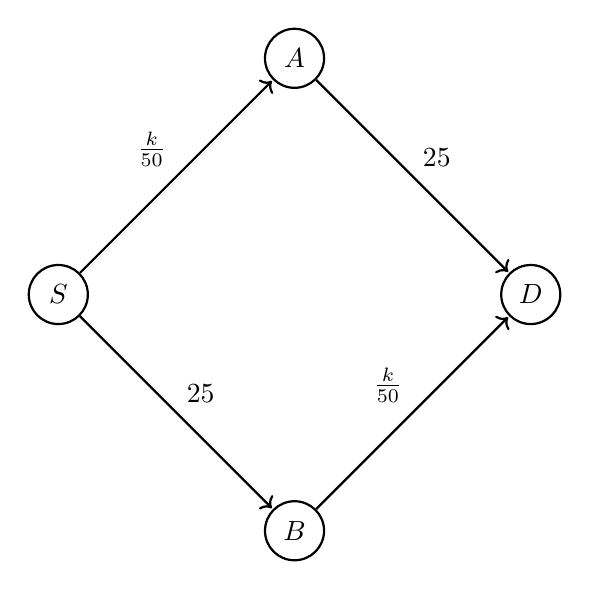
\begin{tikzpicture}[shorten >=0.5pt,node distance=3cm,on grid,auto]
    \tikzstyle{state}=[shape=circle,thick,draw,minimum size=0.75cm]
    \tikzstyle{blank}=[shape=circle, minimum size=0.75cm]

    \node[state] (A1) { $S$};
    
    \node[blank, right of=A1] (B1) {};
    \node[state, right of=B1] (C1) {$D$};
    \node[state, above of=B1] (B0) {$A$};
    \node[state, below of=B1] (B2) {$B$};
    
    
    \path[->,draw,thick]
    (A1) edge node {$\frac{k}{50}$} (B0)
    (A1) edge node {$25$} (B2) 
    (B0) edge node {$25$} (C1)
    (B2) edge node  {$\frac{k}{50}$} (C1)
    ;

  \end{tikzpicture}  \caption{Braess's Paradox : A Transportation Network }
  \label{fig:braess1}
\end{figure}

Consider a strategy where the number of vehicles on both the links is equal. In this case, the total travel time is $35$ minutes.

\bigskip

Now, we introduce another fast path to this network. Consider that we build an expressway (one-way) connecting $A$ to $B$. To simplify, we consider that travel time across this expressway is $0$. This new network is as follows:

\begin{figure}[!h]
  \centering
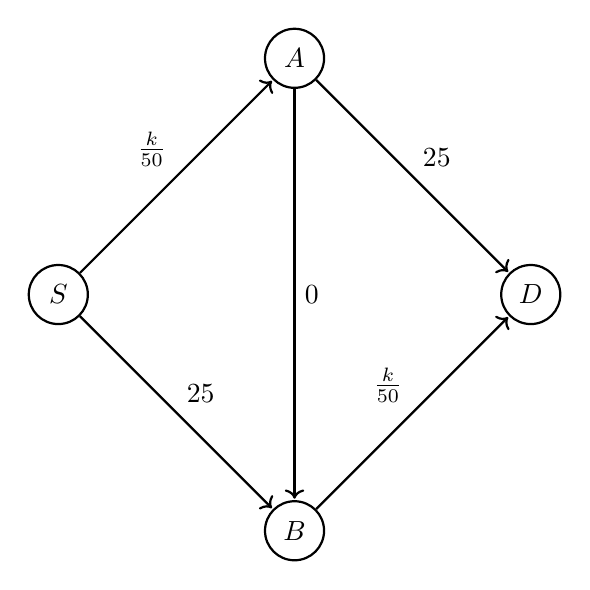
\begin{tikzpicture}[shorten >=0.5pt,node distance=3cm,on grid,auto]
    \tikzstyle{state}=[shape=circle,thick,draw,minimum size=0.75cm]
    \tikzstyle{blank}=[shape=circle, minimum size=0.75cm]

    \node[state] (A1) { $S$};
    
    \node[blank, right of=A1] (B1) {};
    \node[state, right of=B1] (C1) {$D$};
    \node[state, above of=B1] (B0) {$A$};
    \node[state, below of=B1] (B2) {$B$};
    
    
    \path[->,draw,thick]
    (A1) edge node {$\frac{k}{50}$} (B0)
    (A1) edge node {$25$} (B2) 
    (B0) edge node {$25$} (C1)
    (B2) edge node  {$\frac{k}{50}$} (C1)
    (B0) edge node {$0$} (B2)
    ;

  \end{tikzpicture}  \caption{The Transportation Network with an Added Path}
  \label{fig:braess2}
\end{figure}

For this game, path $AB$ is a dominant strategy. Hence, all vehicles choose path $AB$, giving us $n_A = 0, n_B=0, n_{AB} = 1000$ and giving us a travel time of $40$ minutes for each vehicle which is greater than the $35$ minutes we saw for $n_A = n_B = 500$ in the network without $AB$. The catch here is that adding an additional link $AB$ forced everyone to use this path, causing greater congestion. \medskip

To illustrate the Braess's Paradox: In Seoul, South Korea, traffic congestion in the city actually reduced when a high-speed arterial link was closed for traffic in relation with the Cheonggyecheon restoration project. A similar scenario also happened in Stuttgart, Germany. In $1990$ the temporary closing of $42^{\text{nd}}$ Street in New York City for Earth Day reduced the amount of congestion in the area. In $2008$ Youn, Gastner and Jeong pointed out roads in Boston, New York City and London that could be closed to reduce predicted travel times. In $2009$, New York experimented with closures of Broadway at Times Square and Herald Square, which resulted in improved traffic flow and permanent pedestrian plazas.

\subsection{The Two-Thirds Game and K-Level Reasoning}

Consider that you are one amongst a thousand people playing a game. Each of you has to guess a real number between $0$ and $100$. The person whose guess is closest to two-thirds of the average guess wins \rupee~10000 (each, in case of a tie). What number should you guess? \medskip

Note that the average guess cannot be more than $100$. Hence, two-thirds of the average guess cannot be more than $66 \frac{2}{3}$. But, now all the players know that none of the players would guess anything above $66 \frac{2}{3}$. Hence, two-thirds of the average further comes down to $44 \frac{4}{9}$. But now all the players know that nobody would guess above $44 \frac{4}{9}$, hence two-thirds of the average further comes down to $29 \frac{17}{27}$. Doing this iteratively, we find that all numbers above $0$ are eliminated. Thus, the optimal outcome is for all players is to guess $0$. Indeed, if everyone guesses $0$ then two-thirds of the average would also be $0$ and everyone wins. \medskip

Thus, ideally, everyone should guess 0. However, when this game is played in real life with real players, the result obtained is remarkably different from the expected result. The average guess usually falls around $25$ or $26$. This problem illustrates the difference between rationality of one player and common knowledge about rationality of all players. Even if we consider each player to be rational and intelligent, they will select $0$ only if they know that everyone else is rational and intelligent as well. However, this is clearly not true in the real setting. In the real setting, the players operate at different \textit{levels of reasoning}. A level-zero player is one who chooses his number randomly. A level-one player is a player who makes his decision under the assumption that all other players are level-zero players. Since the level-zero players choose randomly, their average would turn out to be roughly $50$. Hence, a level-one player would choose $33 \frac{1}{3}$ as his guess. A level-two player makes his decision under the assumption that all players are level-one players. Hence, a level-two player would guess $22 \frac{2}{9}$. In general, a level-$K$ player would make his decision under the assumption that every player is a level-($K-1$) player. In the real setting, we have a varied distribution of people from different levels which gives us a result different than the one we expected. 


\subsection{The Commitment Problem and Civil Wars}

A commitment problem in Game Theory is a situation where one party promises you a certain outcome but this promise is not credible. Commitment problems can in fact also explain how civil wars begin and why they are so notoriously difficult to end. Consider a situation in a country where the rulers / majority are committing atrocities against the ethnic minorities. At this point, the minorities have two options - whether to start a civil war or whether to wait and see if the situation improves. If the minorities decide to wait and watch, then the government can either continue these atrocities or stop them. The government would prefer if the minorities don't revolt as this would save the wealth and life they would lose due to a civil war. Hence, the government tries to convince the minority that it wouldn't commit atrocities. Although this is a better outcome for both the sides, the government cannot credibly commit to stop atrocities (as it has been committing atrocities up till now). Also, if the atrocities continued, the position of the minorities would only weaken, leaving them with a lesser chance of success if they revolt at a later time. Due to this commitment problem, the minorities decide that it is in their best interest to start a civil war right now. \smallskip

We have talked about how civil wars start due to a commitment problem. What about stopping these wars ? Let us first make a clear distinction between how interstate (involving two or more countries) wars come to an end and how civil wars come to an end. Roughly two-thirds of interstate wars have ended in a negotiated settlement between the sides. They start fighting, learn more about each other and eventually come to a mutually preferable outcome - a settlement. Civil wars, on the other hand, do not follow such a trend. Less than one-fifths of civil wars end in a negotiated settlement. Why? Game Theory answers this question very well. \smallskip

Consider that a civil war is nearing its end. At this point, the minorities have two options - to surrender or to continue fighting. If they continue fighting, then both sides lose more and more of their resources and the civil war continues. If they surrender, the government can decide whether to forgive them or execute them for treason. The government tells the minorities that the government is willing to forgive them and that this outcome is better for both of them. While this is true, imagine what happens when the minorities surrender. They lose all their arms and are rendered powerless. The government is now free to do whatever it wants. It is now the supreme authority and is not obliged to forgive the minorities as they had promised. As they no longer have arms, the minorities wouldn't be able to do anything if the government suddenly decided to execute them. The government therefore cannot credibly commit to forgiving them, and thus, the civil war continues. \smallskip

The critical requirement for a civil war to end is third-party intervention. A third party intervention forces the government/majority to credibly commit, thus resolving the conflict. For peaceful settlement of the conflict, the third party (or the enforcer) must have an interest in a peaceful settlement which will counterbalance the resources it must invest in the enforcement. This could be a financial gain because of stability in the region. Secondly, the enforcer must have enough military power to uphold the enforcement. Thirdly, the enforcer must be unbiased. These conditions rule out most of the countries as effective enforcers. Hence, a lot of civil wars continue. \smallskip

An interstate war is more complicated as there are a lot more players involved. It is not simply a minority versus majority scenario. There are international treaties to hold countries accountable for their actions. Unlike the majoritarian government, neither of the countries are free to do as they will. Their actions are monitored and there are effective enforcers willing to invest in a peaceful settlement. \smallskip

\subsection{Hotelling's Game}

Consider that you are a vendor on a long beach selling ice-cream at some price. Your cart is placed at the middle of the beach. One day, a friend of yours arrives with a cart selling the same ice-cream and at the same price. 
We represent the beach as the interval $[0,1]$ and assume that the beach goers are uniformly distributed over the beach. Both of you agree to split the beach in half with you placing your cart at $0.25$ and he placing his cart at $0.75$. The beach-goers go to the cart which is closest to them. Each of you now serves exactly $50 \%$ of the beach crowd. This solution minimises the distance each beach goer has to walk, and is thus called a socially optimal solution. The next day, your friend sets up his cart exactly in the middle of the beach at $0.5$ while you set up your cart at your usual location of $0.25$. You get the $25 \%$ customers to the left of you and half of the customers between you and your friend's cart. Thus, you serve only $37.5 \%$ of the beach crowd. Your friend gets all the customers to his right as well as half of the customers between your carts. Thus, he serves $62.5 \%$ of the crowd, getting a higher profit. The next day, you arrive earlier than your friend and set up your cart at $0.75$ hoping to get all the customers to your left. But, your friend sets up his cart at $0.74$, stealing all your customers leaving only a short fraction of customers to you. To overcome this, you move slightly to the left of your friend, to $0.73$. He wishes to regain his customers and so, moves to $0.72$. You move to $0.71$ and this process goes on. It then happens that both of you have set up your cart exactly at $0.5$. At this point, neither of you would want to shift your position given that the other is still at $0.5$. Hence, both of you have reached a Nash equilibrium. This phenomenon is known as Hotelling's Model of Spatial Competition, or the Hotelling's Game in short. This phenomenon also explains why competitor stores like pizza places, coffee shops, etc. open their stores next to each other and occur in clusters rather than being uniformly distributed. 

\subsection{Modelling COVID-$19$ as a Game}

We can think of the current pandemic situation cause by COVID-$19$ to be a game. This is nothing but a strategic interaction between us, the society, and the virus. In particular, the nature of the game is such that the virus attacks us, and then we interact with one another. There are three key sets of players in this game - the virus, the society and the policymakers (who control the level of interaction within society). The payoff to the virus is simple - it wants to infect more and more people. The payoffs to us are considerably more complicated - these are a combination of health effects and economic effects. Moreover, the level of these effects are different for different sections of society. For example, a daily wage worker would be more concerned with economic effects than a middle-class person. \medskip

We can further divide the society into two types - responsive and non-responsive. The responsive section takes precautions like social distancing, sanitation. The non-responsive section proceeds with life with complete normalcy. This game can be modeled as a continuous game - one where people's strategies keep changing with time. For example, the people decide whether to be responsive or non-responsive based on \textit{risk perception}. If the headlines of the news tell them that this virus is dangerous and one must stay indoors then a large number of people would tend to be responsive. Whereas, if they feel that the risk of the virus is overstated, they would tend to be more non-responsive. \medskip

The objective of this game is to survive the pandemic, and break the chain of the virus with minimum damage to economy. Examples around the world have shown us that social distancing and lock-downs have helped in curbing the spread of the virus. The downside however is that a lock-down also adversely affects economy. Moreover, we cannot lift the lock-down frivolously as the virus infects exponentially. Hence, this is a tricky game to play as any form of complacency leads to a sudden spike of cases. How we proceed with this situation remains to be seen. One thing is clear - this is a game we cannot afford to lose. \href{https://drive.google.com/file/d/1gdy970kVrz_XsAbDqjyGGLMZhqzcWYo8/view?usp=sharing}{Here} is a document which discusses the setup of this game.

\subsection{Oligopoly Behaviour and Repeated Prisoner's Dilemma}

An oligopoly is a state where a market is shared by a small number of competitors. In an oligopoly, each firm has several strategic choices - increasing or decreasing the prices of certain products, introducing new products, trying out new marketing strategies. For example, an airline's decision to increase its ticket prices is a strategic choice. The response of the rival airline to this decision is also a strategic choice. The interdependence of these strategic choices strongly influences oligopoly behaviour around us. \medskip

We wish to try to model oligopoly behaviour as a game of prisoner's dilemma. However, there are some obvious obstacles. The prisoner's dilemma is played only once. Each player makes a single choice and the game ends after the first round. In reality, oligopoly involves multiple rounds and multiple strategic choices - a firm raises its price, another firm introduces a new product, the first firm cuts its price, a third firm introduces a new marketing strategy, and so on. For simplicity, we consider a duopoly - an oligopoly involving only two firms. We consider the scenario of a pricing war.  \medskip

Consider that two firms $A$ and $B$ have reached an agreement which lays down the prices for their products. As long as each firm upholds the agreement, it guarantees maximum economic profit to both of them. However, each firm has an incentive to `cheat' on the agreement. If a firm slashes its prices while the other firm maintains it, it could gain a larger share of the market and increase its profit. However, both firms cheating leads to a loss for both of them. Consider that each firm earns economic profits of $20,000$ dollars per month. A payoff matrix for this scenario is given in Table \ref{table:duopoly}. The values represent the gain/loss in thousands of dollars per month that this pricing war is played. 

\begin{table}[H]
    \begin{adjustbox}{width=5cm,center}
    \begin{tabular}{|c|c|c|}
        \hline
        A \textbackslash \: B & Cheat & Not Cheat \\
        \hline
        Cheat & -5,-5 & 8,-8 \\
        \hline 
        Not Cheat & -8,8 & 0,0  \\
        \hline
    \end{tabular}
    \end{adjustbox}
    \caption{Payoff Matrix for the pricing war in a Duopoly}
    \label{table:duopoly}
\end{table}

Cheating is a dominant strategy for both of them. However, this leads to an unfavourable outcome for both of them. They both want to maximise their profits yet each is likely to choose a strategy inconsistent with this goal. If this continued throughout, each firm would drive down prices to their costs itself, leaving each firm with zero profit. However, this is solved by introducing certain new strategies related to repeated prisoner's dilemma. \medskip

One way to encourage cooperation is for both firms to use a \textbf{tit-for-tat} strategy. Each firm responds to cheating by cheating and each firm responds to cooperation by cooperating. As the game progresses, the firms get to know of each other's tit-for-tat strategies and cheating becomes less and less likelier. A tit-for-tat strategy works well as it is both retaliatory as well as forgiving. \medskip

Another way firms may seek to force rivals to behave cooperatively rather than competitively is to use a \textbf{trigger} strategy. In a trigger strategy, a firm threatens to permanently revoke the agreement if the other firm ever cheats. A firm might, for example, make a credible threat to cut prices down to the level of average total cost—and leave them there—in response to any price-cutting by a rival. A trigger strategy is calculated to impose huge costs on any firm that cheats. A firm might threaten to invoke a trigger in hopes that the threat will forestall any cheating by its rivals.

\subsection{The Cold War}

Another example of the trigger strategy was seen in the Cold War between the United States and the Soviet Union. This was a time when both these countries were sitting on stockpiles of nuclear weapons, sufficient to destroy one another many times over. Thomas Schelling suggested that nuclear weapons should not be considered as ordinary weapons, but rather, as \textit{deterrents}. During the Cold War, both sides adopted a strategy known as the \textbf{Mutual Assured Destruction} doctrine or the MAD doctrine. Under the MAD doctrine, each country threatened to launch sufficient nuclear attacks to destroy the other country if the other country launched a nuclear attack against it or one of its allies. The MAD doctrine seems, well, mad as each country was committed to destroy all of humanity for the sake of revenge. However, it worked well and the two nations did not go to war for over $40$ years. Thus, the MAD doctrine was indeed an effective trigger strategy.


\section{Quantum Game Theory}

Quantum Game Theory is perhaps the most ambitious crossover in science - that of Classical Game Theory and Quantum Mechanics. Quantum Game Theory analyses classical games in the quantum domain and with added `quantum effects'. A quantum game differs from a classical game in three primary ways 
\begin{enumerate}
    \item Superposed initial states
    \item Entanglement of initial states
    \item Superposition of strategies to be used on initial states
\end{enumerate}
A detailed study of Quantum Game Theory is highly involved. However, I provide a simple example giving a glimpse of the wonders that quantum mechanics brings to Game Theory. We introduce a \textit{Quantum Prisoner's Dilemma}. \medskip

In the quantum variant of the Prisoner's Dilemma, the outcome is a $2$-dimensional qubit in the vector space spanned by the orthonormal vectors $\{ \ket{C}, \ket{D} \}$, where $\ket{C}$ corresponds to cooperate and $\ket{D}$ corresponds to defect. The first qubit corresponds to player $A$'s decision and the second one to player $B$'s. Thus, the outcome space is the set $\{ \ket{CC}, \ket{CD}, \ket{DC}, \ket{DD}\}$.\footnote{Note: I have used $\ket{CC}$ as a succinct expression for $\ket{C} \otimes \ket{C}$ and similarly for each pair.} Initially, both the qubits start as $\ket{C}$ and are passed through a unitary gate $\hat{\mathcal{J}}$. This gate (called the \textbf{entanglement gate}) can provide varied degrees of entanglement, based on a parameter, $\gamma$, called the \textit{entanglement degree}. The output then goes through two gates $\hat{U}_A$ and $\hat{U}_B$ where these gates correspond to matrices chosen by players $A$ and $B$ to decide their strategy. Classically, they can choose either 
\[
    C = 
    \begin{pmatrix}
    1 & 0 \\
    0 & 1
    \end{pmatrix} \quad 
    D = 
    \begin{pmatrix}
    0 & 1 \\
    -1 & 0
    \end{pmatrix}
\]
corresponding to $\ket{C}$ and $\ket{D}$ respectively. In the quantum game, these matrices can be any unitary matrices. Finally, the output is passed through another gate $\hat{\mathcal{J}^{\dagger}}$ and then measured to calculate the payoffs. This can be compactly represented as the circuit shown in Figure \ref{fig:qpd}. $\ket{\psi_0}$ and $\ket{\psi_f}$ are the initial and final states respectively. The final outcome is given by
\[
    \ket{\psi_f} = \hat{\mathcal{J}^{\dagger}}\left( \hat{U}_A \otimes \hat{U}_B \right) \hat{\mathcal{J}} \ket{CC}
\]

\begin{figure}[h!]
    \centering
    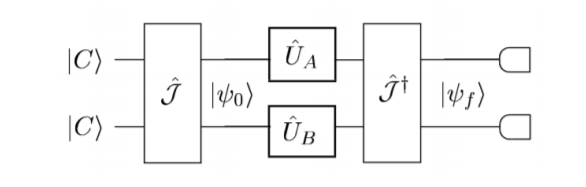
\includegraphics[scale=0.5]{qpd.png}
    \caption{Quantum Prisoner's Dilemma Circuit}
    \label{fig:qpd}
\end{figure}
\medskip

When $\hat{\mathcal{J}}$ provides no entanglement, the classical result still remains. That is, $D \otimes D$ is the Nash equilibrium for this game. However, when we introduce entanglement between the qubits, things change. If player $B$ plays $D$ then player $A$'s best strategy is no longer $D$, but is the unitary matrix $Q$ given by 
\[
    Q = 
    \begin{pmatrix}
    \iota & 0 \\
    0 & -\iota
    \end{pmatrix}
\]  
However, once we allow both players to use quantum strategies, we see that both players would play a meta-strategy (a classical mixture of quantum strategies) which leads to a constant sum game. Thus, there are \textit{infinitely many equilibria} in the Quantum Prisoner's Dilemma. Entanglement cause an intrinsic correlation between cooperation and defection outcomes. Each player's strategies are inherently affected by the other's strategy leading to a matching-pennies style scenario. This quantum approach to games finds extensive use in economics, cryptography and often performs better than a classical approach.

\section{Evolutionary Game Theory}

\subsection{Introduction and Evolutionarily Stable Strategies}

Another interesting application of Game Theory is the branch of Evolutionary Game Theory (EGT). EGT is the application of Game Theory in the study of evolving populations in biology. The field of EGT was primarily developed by mathematical biologist John Maynard Smith. He realised that an evolutionary version of game theory does not require rationality of the players (as opposed to classical game theory). It only requires that the players have a strategy. How good the strategy was is shown by the results of the game, just as how evolution tests alternate strategies for the ability to survive and reproduce. The participants in an evolutionary contest have the ultimate aim of producing as many replicas of themselves as possible. The payoff is in units of fitness (called \textbf{Darwinian fitness}). The fitness of an organism represents how well it does or how likely it is to survive in competitive environments. The success of an organism thus depends on how its behaviour interacts with those of its competitors. This notion of fitness and behaviour leads to an immediate game-theoretic interpretation. We consider an organism's genetic traits and behaviour to be its strategy. An organism's payoff (fitness) is then dependent on its own as well the strategy of all its competitors (just as a game).\medskip

The test for the stability of a population is its resistance to the introduction of mutants. If the introduction of a mutant strategy allows the mutants to grow their population then we say that they \textit{invade} the population. A population where no other mutant strategy can enter and disturb the population dynamics is called an \textbf{evolutionarily stable strategy (ESS) }. An ESS is a strategy that is resistant to invasion.

\subsection{How Genetic Traits Become Strategies}

Suppose there are two species of beetles - large beetles and small beetles. They often contest over food and nutrients. When two beetles of the same size contest, they share the food. If a large beetle contests with a small beetle then it gets all the food. However, the payoff (in terms of fitness) that the large beetles get from a particular quantity of food is actually less as it requires more food to maintain its metabolic requirements (due to a larger size). The payoff matrix for this is shown in Table \ref{table:beetle}.

\begin{table}[H]
    \begin{adjustbox}{center}
    \begin{tabular}{|c|c|c|}
        \hline
         1 \textbackslash \; 2 & Small & Large \\
        \hline
        Small & 5,5 & 1,8 \\
        \hline 
        Large & 8,1 & 3,3  \\
        \hline
    \end{tabular}
    \end{adjustbox}
    \caption{Payoff Matrix for the Beetles Game}
    \label{table:beetle}
\end{table}

These numerical payoffs satisfy our conditions. The key difference from classical game theory here is that the beetles do not have any control of their body size and are genetically hard-wired to play a single strategy throughout their lifetime. Notice that the Large strategy is a strictly dominant strategy and hence, it is an ESS. We can also explain this analytically. If we start off with a $100\%$ small beetle population and introduce a few large beetles then the large beetles would do exceedingly well, winning every contest \footnote{While introducing mutants, we ignore their interactions with each other as these are sufficiently rare and can be neglected}. If we introduced a few small beetles in a $100\%$ large beetle population then they would do terribly, losing every contest. This situation is exactly the same as the Prisoner's Dilemma. While the Small-Small outcome is a mutually better outcome than the Large-Large outcome, it is unstable to the introduction of large beetles. \medskip

A similar analogy is also applicable to the heights of neighbouring trees.  If both trees grow short, they share the sunlight equally. If they both grow tall then they again share the sunlight equally but the same amount of sunlight is now less valuable as they have a larger size. However, a tall tree growing beside a short tree takes up all the sunlight. These strategies are akin to the small and large strategies in beetles. However, the actual scenario is much more complex as it involves a continuum of strategies. We then look for a `threshold', beyond which a further increase of the height/size cannot be compensated by added advantages of resources. \medskip

\subsection{Mathematical Treatment of Evolutionary Stable Strategies}

We now consider a general evolutionary game and draw comparisons between an ESS and a Nash equilibrium. Consider that an organism has two variants - $S$ and $T$. A payoff matrix for its contest with another organism is shown in Table \ref{table:ess}.

\begin{table}[H]
    \begin{adjustbox}{center}
    \begin{tabular}{|c|c|c|}
        \hline
         1 \textbackslash \; 2 & S & T \\
        \hline
        S & a,a & b,c \\
        \hline 
        T & c,b & d,d  \\
        \hline
    \end{tabular}
    \end{adjustbox}
    \caption{Payoff Matrix for a Symmetric Evolutionary Game}
    \label{table:ess}
\end{table}

Let us find the condition for $S$ to be an ESS. We consider that only a small fraction $x >0$ of the population is of $T$ variant. The expected payoff for an $S$ variant is then $a(1-x) + bx$ while the expected payoff for a $T$ variant is $c(1-x) + dx$. Therefore, $S$ is an ESS if for sufficiently small $x$, the following inequality holds
\[
    a(1-x) + bx > c(1-x) + dx
\]
As $x$ goes to zero, we must have $a > c$. However, if $a=c$, then we must have $b>d$. Thus, $S$ is an ESS precisely when either $(i)\; a > c$ or $(ii)\; a=c$ and $b>d$. Further, if $S$ is an ESS, then the outcome $(S,S)$ is a Nash equilibrium. However, the converse does not hold. For example, a scenario where $a=c$ and $b<d$ is a Nash equilibrium but $S$ is not an ESS. It is interesting to note that the Nash equilibrium and ESS share close similarities despite being built in different contexts. The Nash equilibrium demands players to be rational and capable of calculating their optimal strategies. However, an ESS makes no such demand and naturally selects strategies which are more successful.


\subsection{The Hawk-Dove Game}

So far we have only considered pure strategy equilibria. Let us also introduce the notion of mixed strategies in evolutionary games. We study the Hawk-Dove Game, a classic example in EGT which models a contest over a shareable resource. The contestants can either be hawks or doves. The hawk first displays aggression, then escalates it into a fight until it either wins or is injured (loses). The dove first displays aggression but if it faced with a fight, it flees. If not, it tries to share the resource. Consider that the value of the resource is $V$(that is, the fitness of a contestant increases by $V$ if it acquires the resource) and the cost of losing a fight is $C$ (that is, the fitness of a contestant decreases by $C$ if it loses a fight). Thus, the following outcomes are possible 

\begin{itemize}
    \item If a Hawk meets a Dove, then he keeps all the resource to himself ($V$)
    \item If a Hawk meets a Hawk, then he wins and loses with equal probability - thus his average outcome is $\frac{V}{2} - \frac{C}{2}$
    \item If a Dove meets a Hawk, then he backs off and gets nothing ($0$)
    \item If a Dove meets a Dove, then they share the resources ($\frac{V}{2}$)
\end{itemize}

The payoff matrix for this is given in Table \ref{table:hd}.

\begin{table}[H]
    \begin{adjustbox}{center}
    \begin{tabular}{|c|c|c|}
        \hline
         & meets Hawk & meets Dove \\
        \hline
        if Hawk & $\nicefrac{V}{2} - \nicefrac{C}{2}$ & $V$\\
        \hline 
        if Dove & $0$ & $\nicefrac{V}{2}$  \\
        \hline
    \end{tabular}
    \end{adjustbox}
    \caption{Payoff Matrix for the Hawk-Dove game.}
    \label{table:hd}
\end{table}

However the actual payoff actually depends on the probability of one strategy meeting the other, which in turn, is representative of their percentages in the population. These percentages are in turn determined by the results of all the previous such contests. If the cost of losing $C$ is more than the value of the resource $V$ (as is in the natural world) then the population dynamics ends with Hawks having a fraction $\frac{V}{C}$ . To arrive at this conclusion, let us start with a $100\%$ Hawk population and consider that we have introduced a very small population of doves. When, hawks fight with hawks, their fitness actually decreases (as $V < C$) but the doves don't incur any cost (called a `neutral allele') when they meet hawks and their fitness remains the same. Hence, the doves grow in population and a pure-hawk strategy isn't evolutionarily stable. Now consider a population of all doves and we introduce a few hawks. The doves increase their fitness by only $\frac{V}{2}$ when they contest amongst themselves. However, hawks increase their fitness by $V$ while contesting with doves. Hence, the hawks grow in population and a pure-dove strategy isn't evolutionarily stable. Thus, the evolutionarily stable strategy must be in a mixed strategy. Further calculations gives us the optimal fraction of hawks to be $\frac{V}{C}$. \medskip

There are two ways to interpret mixed strategies in an evolutionary game. Firstly, we can think of the distribution being representative of the distribution of pure species in the population. For example, the outcome of the Hawk-Dove game can be interpreted as a fraction $\frac{V}{C}$ being hawks and the others being doves. Another interpretation is that each member in the population is genetically the same and is genetically hard-wired to choose a mixed strategy where he plays a hawk-like strategy with probability $\frac{V}{C}$.

\subsection{Virus Mutations}

We have studied both the evolutionary prisoner's dilemma as well as the hawk-dove game. We apply these ideas to a real biological scenario. \medskip

Another interesting application of the Evolutionary Prisoner's Dilemma is in virus populations. This was a study conducted by Turner and Chao where they studied the virus Phage $\Phi6$ which infects bacterial hosts and produces chemicals necessary for their survival. A mutational variant of this virus, Phage $\Phi \text{H}2$ can also replicate in bacterial hosts though less effectively on its own. But in the presence of $\Phi6$, $\Phi \text{H}2$ can use up the chemicals produced by $\Phi6$ giving them a fitness advantage over $\Phi6$. When there is a pure population present, $\Phi6$ does better than $\Phi \text{H}2$. However, a virus is always better off being of type $\Phi \text{H}2$ regardless of its environment. Hence, $\Phi \text{H} 2$ is an ESS. They measured relative rates of the growth of the virus variants and came up with the following payoff matrix, shown in Table \ref{table:virus1}.

\begin{table}[H]
    \begin{adjustbox}{center}
    \begin{tabular}{|c|c|c|}
        \hline
         1 \textbackslash \; 2& $\Phi6$ & $\Phi \text{H} 2$ \\
        \hline
        $\Phi6$ & 1.00, 1.00 & 0.65, 1.99\\
        \hline 
        $\Phi \text{H} 2$ & 1.99, 0.65 & 0.83, 0.83  \\
        \hline
    \end{tabular}
    \end{adjustbox}
    \caption{Payoff Matrix for the Virus Game}
    \label{table:virus1}
\end{table}

However, there is a very thin line that separates an Evolutionary Prisoner's Dilemma from a Hawk-Dove game. Consider, for example that the variant $\Phi \text{H} 2$ didn't survive on its own as well as it did in the previous example. The modified payoff matrix is then as shown in Table \ref{table:virus2}.

\begin{table}[H]
    \begin{adjustbox}{center}
    \begin{tabular}{|c|c|c|}
        \hline
         1 \textbackslash \; 2& $\Phi6$ & $\Phi \text{H} 2$ \\
        \hline
        $\Phi6$ & 1.00, 1.00 & 0.65, 1.99\\
        \hline 
        $\Phi \text{H} 2$ & 1.99, 0.65 & 0.50, 0.50  \\
        \hline
    \end{tabular}
    \end{adjustbox}
    \caption{Payoff Matrix for the Modified Virus Game}
    \label{table:virus2}
\end{table}

This game now has a Hawk-Dove structure rather than a Prisoner's Dilemma structure. Thus, the final outcome is a co-existence of both the variants of the virus. We see how slightly tweaking the numbers can decide whether a species can co-exist or is driven to extinction. In both structures, a player can choose to be `helpful' or `selfish'. In the Prisoner's Dilemma, penalties for selfishness are mild and hence both players behave selfishly. In the Hawk-Dove, however, selfishness is sufficiently harmful for both players and thus, at least one player tries to avoid it. 


\section{Voting and Group Decision Making}

\subsection{Introduction and Condorcet's Paradox}

We have seen voting all around us, be it the General or State elections, the jury voting on a verdict, a legislative assembly voting on whether to pass a bill. Essentially, a voting system (or an aggregation procedure) is a mechanism to aggregate information across a group. More concretely, a voting system takes in a collection of complete and transitive (or rational) individual preferences and produces \textit{group ranking} of the outcomes. With such a general definition, it is hard to understand what makes a `reasonable' voting system. We start with the most common (and the most natural) one - \textit{majority rule}. \medskip

When there are two alternatives, under majority rule, we take the alternative preferred by majority of the voters and rank it first. The other alternative is ranked second. While this seems natural, extending it to multiple alternatives is problematic, as we shall illustrate with \textbf{Condorcet's Paradox}, named after Marquis de Condorcet, a French political philosopher. Condorcet's Paradox states that while individual preferences in a group may be rational, they need not lead to a rational group preference. Consider that Donald, Marco and Ted are deciding between three outcomes $A,B$ and $C$. Donald has the preference $C \succ A \succ B$. Marco has the preference $A \succ B \succ C$. Ted has the preference $B \succ C \succ A$. Each of their preferences are complete and transitive, hence they are all rational. Let us decide the group preference according to the majority rule. If more individuals prefer x to y, then the group as a whole prefers x to y. Consider A vs B. Donald and Marco both prefer A to B. Hence, by majority rule, the group prefers A to B. Similarly, we get, B to C and C to A. But this does not obey transitivity. Individual preferences with transitivity were converted into a group preference without transitivity. This is a paradox because the majority interests clash with each other. The majority prefers $A$ to $B$, $B$ to $C$ and yet the majority also prefers $C$ to $A$. Thus, even though the individual preferences formed a \textit{ranking order}, we cannot find a suitable group ranking. \medskip

There are multiple ways of how we could use the majority rule to choose a winner. For example, we can arrange all the alternatives in some order and then eliminate them one-by-one in that order. That is, we compare the first two alternatives and eliminate one via majority vote. The winner is paired with the third alternative and one is eliminated via majority vote. This way, the winner of the last contest is declared the group-favourite. Another way to do this is to create a binary tree out of the alternatives. The winner of each pair of terminal nodes moves one `level' up. In this way, the alternative which reaches the root node is declared the group favourite. This is similar to a knock-out stage in many tournaments. However there are still many problems in this method. In the above example, if we paired $A$ and $B$ first and then paired the winner with $C$, then the group favourite turns out to be $C$. However, if paired $B$ and $C$ and then paired the winner with $A$, the group favourite turns out to be $A$, which is problematic as a group favourite must be independent of the ordering or structure of the mechanism. Condorcet's paradox also captures pathalogies in a single individual's ranking, evaluated over multiple criteria (that is, a person prefers one outcome over the other if he/she prefers majority of the criteria in that outcome).

\subsection{Positional Voting}

Another voting system is one which assigns weights or `points' to alternatives based on their ranking in each individual's preference. A simple example of this system is the \textbf{Borda count} system, proposed by French mathematician Jean Charles de Borda. If there are $k$ alternatives in total, then each individual's ranking confers $k-1$ points on her first alternative, $k-2$ on her second alternative all the way down to $0$ points on her last alternative. The total points of a particular alternative is then the sum of points of that alternative in each individual's ranking. For example, if we have two voters $1$ and $2$ who have the preference relation
\[
    A \succ_1 B \succ_1 C \succ_1 D
\]
\[
    B \succ_2 C \succ_2 A \succ_2 D
\]
over four alternatives. The cumulative points of $A$ are $4$, $B$ are $5$, $C$ are $3$ and $D$ are $0$. Thus, the group ranking is
\[
    B \succ A \succ C \succ D
\]
Some variants of the Borda count exist, such as one where the points range from $1$ to $k$ instead of $0$ to $k-1$ (the system starting at $1$ is in fact used in Slovenian parliamentary elections). Another variant is called the \textbf{Dowdall system}, which assigns points $1$ to the first alternative, $\frac{1}{2}$ to the second alternative, $\frac{1}{3}$ to the third alternative, all the way to $\frac{1}{k}$ to the last alternative. An advantage of the Borda count is that it always produces a rational ranking order (which may have ties). \medskip

However there are problems with the method of Borda count as well. Consider $5$ voters ranking two outcomes $A$ and $B$. Voters $1$ to $3$ prefer $A$ to $B$, while voters $4$ and $5$ prefer $B$ to $A$. The Borda count (and also the majority vote) produces $A$ as the group winner here. Consider now that we add a third alternative $C$. Voters $1$ to $3$ now have the preference order
\[
    A \succ B \succ C
\]
and voters $4$ and $5$ have the preference order
\[
    B \succ C \succ A
\]
Borda count actually produces $B$ as the winner for this preference order. Notice how the introduction of a third alternative (which is in fact lesser preferred than the other two) changes the group winner, while logically it should have remained the same as the introduction of an (irrelevant) alternative $C$ shouldn't affect the group's preference between $A$ and $B$. Further, this poses another problem. Suppose that voters $4$ and $5$ in fact had the preference order
\[
    B \succ A \succ C
\]
In this case, Borda count produces $A$ as the winner. However, voters $4$ and $5$ could \textit{strategically misreport} their preference as $B \succ C \succ A$ to get the winner of their choice. Thus, voters can sometimes benefit by lying about their preferences (essentially by bringing down the competitor to their favourite). We are already seeing how subtle and simple principle in Game Theory explain common political strategies and tactics. \medskip

\subsection{Arrow's Impossibility Theorem}

We must all ask one question at this point - is there \textit{any} voting mechanism which avoids all these pathologies and is truly fair? Any fair voting system must satisfy two crucial properties 
\begin{enumerate}
    \item \textit{Unanimity.} If for a pair of every alternatives $X$ and $Y$, if every individual of a group prefers $X$ to $Y$ then the group as a whole must also prefer $X$ to $Y$.
    \item \textit{Independence of Irrelevant Alternatives (IIA).} For each pair of alternatives, the ordering of $X$ and $Y$ in the group ranking must only depend on how each individual ranks $X$ and $Y$ \textit{relative} to each other. That is, as long as the relative order of $X$ and $Y$ remains same in each individual order (regardless of their actual positions), then the group ranking must have the same preference between $X$ and $Y$.
\end{enumerate}

For two alternatives, we see that the majority rule satisfies both these conditions. However, neither the positional voting system or the majority rule satisfies these conditions for three or more alternatives. However, there is one voting system which satisfies these conditions - dictatorship. A dictatorship is a system where we pick one individual out of the $k$ voters and declare his individual preference as the group ranking. \medskip

Arrow's Theorem states that if there are at least three alternatives then there is no voting system that satisfies unanimity, IIA and is non-dictatorial. Thus, every non-dictatorial voting system is subject to unavoidable trade-offs. Keeping this in mind, we must now focus on managing these trade-offs. Note that the premises of the difficulties posed by Condorcet's paradox and Arrow's theorem often don't arise in real-life scenarios. Consider the preference relations we specified in Condorcet's paradox. Consider that $A$, $B$ and $C$ are political candidates with $A$ being liberal, $B$ being moderate and $C$ being conservative. Marco prefers the liberal candidate to the moderate candidate to the conservative candidate. Ted prefers the moderate candidate to the conservative candidate to the liberal candidate. Both these preference orders seem ``sensible''. We can explain them via a sense of `proximity' to an ideal choice. For example, Marco is liberal leaning and hence his preference order is the order in which the alternatives are `close' to being liberal. Ted is fairly centrist (slightly conservative leaning) and prefers the moderate candidate. However, if he had to choose between the two extremes, he would prefer the conservative candidate, who is closer to his leaning. However, Donald prefers the conservative candidate to the liberal candidate to the moderate candidate. Clearly, this doesn't seem to make sense. If Donald leans conservative, then he should (ideally) prefer the moderate candidate over the liberal one. Note that this is not a `wrong' preference but is rather unusual. We now try to formalise this ``unusualness'' of preferences.

\subsection{Single-Peaked Preferences and the Median Voter Theorem}

The general idea of reasonable preferences is that each voter has a favourite alternative and his/her preference for alternatives decreases as the alternatives move farther away from the favourite. Suppose there are $k$ (ordered) alternatives, $X_1, \ldots , X_k$. We say ordered alternatives as there is a natural way of arranging them in some orderly fashion (for example, we can arrange political candidates on a political spectrum). We say that a voter has \textbf{single-peaked preferences} if there is no alternative $X_s$ such that the two neighbouring alternatives $X_{s-1}$ and $X_{s+1}$ are both ranked above $X_s$. That is, the voter never prefers two options that lie on opposite sides of a middle option. This is equivalent to saying that each voter has a favourite alternative $X_t$ and his preference relation then has the form
\[
    X_1 \prec X_2 \prec \ldots \prec X_{t-1} \prec X_t \succ X_{t+1} \succ \ldots \succ X_{k-1} \succ X_k
\]
Some examples of single-peaked preferences are shown in Figure \ref{fig:spp}.

\begin{figure}[h!]
    \centering
    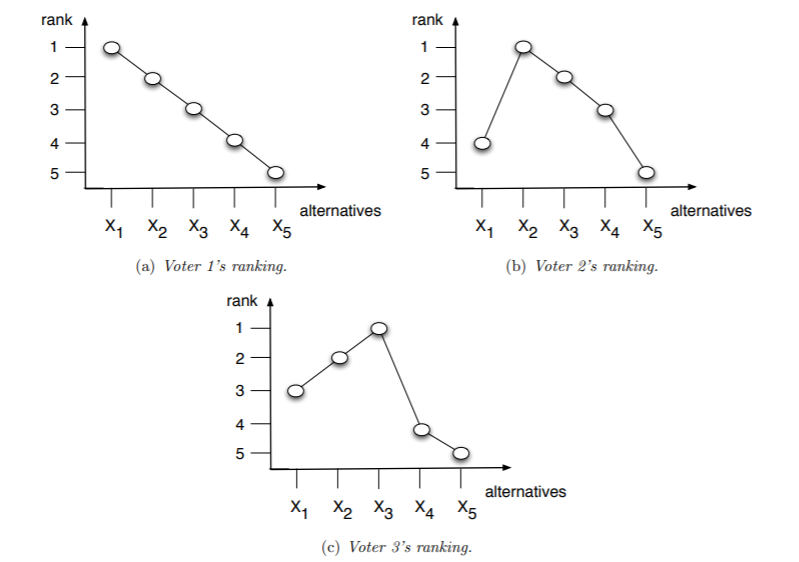
\includegraphics[scale=0.6]{SPP.png}
    \caption{Examples of single-peaked preferences}
    \label{fig:spp}
\end{figure}

Having studied single-peaked preferences, we now claim the following. If all individual preferences are single-peaked then applying majority rule pairwise produces a group relation which is both complete and transitive. Let us choose the group favourite. Suppose we line up all individual favourites in the natural order. Intuitively, the group favourite would be the one in the middle (the median) as this alternative naturally ``compromises'' between the extreme alternatives. \medskip

The Median Voter Theorem states that with single-peaked preferences, the median individual favourite is also the group favourite. Let $X_m$ be the median individual favourite. Any other alternative $X_t$ must lie on one side of $X_m$. Without loss of generality, assume that $X_t$ lies to right of $m$ (we can always reverse the order). Now, each voter whose individual favourite is to the left of $X_m$ would prefer $X_m$ over $X_t$ as its closer to their favourite alternative. Exactly half of the electorate lies to the left of $X_m$. The median voter himself chooses $X_m$ (which happens to be his own favourite). Hence, $X_m$ has a majority over any other alternative. Note how this is similar to the Hotelling's game where both ice-cream vendors tried to get as close to the ``center'' as possible. The idea is the same with the center being the median individual favourite. After a group favourite has been chosen, we remove that alternative from the ranking of every player and re-choose a group favourite. This gives us the second favourite. Continuing this way, we can rank all the alternatives rationally.

\section{Auctions}

\subsection{Introduction}

Another interesting scenario where Game Theory is that of auctions. For single-item auctions, there are four main types of auctions - 
\begin{itemize}
    \item \textit{Ascending-Bid Auctions (English Auctions).} In this form of auction, the bidders start off at a base price (prescribed by the seller) and the seller gradually raises the price of the item until all but one bidder is willing to pay. 
    \item \textit{Descending-Bid Auctions (Dutch Auctions).} In this form of auction, the seller starts off at a high price and gradually starts to decrease the price of the item until one bidder is willing to pay the price.
    \item \textit{First Price Sealed-Bid Auctions.} In this form of auction, all bidders simultaneously submit ``sealed bids'' to the seller. The bidder with the highest bid wins the auction and buys the item at the value he bid.
    \item \textit{Second Price Sealed-Bid Auctions (Vickrey Auctions).} This is similar to the first price auction. However, the winner of the auction does not pay his own bid but pays the second highest bid for the item.
\end{itemize}

Auctions are generally used by sellers in scenarios where they do not have an estimate of the price that each bidder values the item at. That is, the valuation of the item is \textit{private information}. In such cases, auctions can be used to elicit bids from buyers that reveal these values. The true essence of auctions is only when there is private information. To show this, let us consider a scenario of known values. Let's say that the seller is willing to sell an item at a value of $x$ and the highest bidder is willing to pay $y$ for the item. In this scenario, there is a \textit{surplus} of $y-x$. If these values are known to everyone then the seller can simply declare the price of the item to be just lower than $y$. The highest bidder buys the item at this price and the seller gains nearly all of the surplus. Hence, there is no need for an auction in this scenario as the seller can gain as much as he reasonably expects by just announcing the right price. Here, the seller has complete control over the design or the `mechanism' of the transaction. Imagine instead that the highest bidder could propose a price he is willing to pay for the item. He would propose a price just above $x$ and gain nearly the entire surplus of $y-x$. Thus, the person who has control over the mechanism of the transaction gains the surplus (we call this \textbf{proposal power} in bargaining theory).

\subsection{Second Price Auctions}

In second-price auctions, it is a dominant strategy to make a bid exactly equal to what you value the item at. For each player $i$, let $v_i$ denote bidder $i$'s true value of the item. Let $b_i$ denote the bid made by bidder $i$. The payoffs for this auction are as follows
\begin{enumerate}
    \item If $b_i$ is not the winning bid, then the payoff to $i$ is $0$.
    \item If $b_i$ is the winning bid and $b_j$ is the second highest bid then the payoff to $i$ is $v_i - b_j$.
\end{enumerate}
Our claim is that it is a dominant strategy for $i$ to bid a value $b_i = v_i$. To prove this, we assume $b_i = v_i$ and show that no deviation can produce a higher payoff. Note that changing the value of $b_i$ only decides whether $i$ loses or wins and does not affect the price of the item if he wins (as we only assume unilateral deviations, the second price will remain the same). Consider that the player bids $b^{\prime}_i > v_i$. This only affects the payoff of bidder $i$ if he loses the auction with $v_i$ and wins with $b^{\prime}_i$. In this case, the second highest bid $b_j$, must be between $v_i$ and $b^{\prime}_i$. Thus, the payoff $v_i - b_j \leq 0$, which does not improve $i$'s payoff. Now consider that the player bids $b_i^{\prime \prime} < v_i$. This affects the payoff to $i$ only if he wins with $v_i$ but loses with $b_i^{\prime \prime}$. For a second bid of $b_k$, the original payoff was $v_i - b_k \geq 0$ and the new payoff is $0$. Hence, this doesn't improve $i$'s payoff either. Hence, $b_i = v_i$ is a dominant strategy. This simple argument holds because your bid only decides whether you win or lose and not how much you pay. However, things become much more complex in first-price auctions.

\subsection{First Price Auctions}

In first-price auctions, your bid not only decides whether you win or lose but also how much you pay. The payoffs in a first-price auction are
\begin{enumerate}
    \item If $b_i$ is not the winning bid, then the payoff to $i$ is $0$.
    \item If $b_i$ is the winning bid, then the payoff to $i$ is $v_i - b_i$.
\end{enumerate}

Note immediately that if you bid your true value then your payoff is $0$ regardless of whether you win or lose. Your optimal strategy is therefore to bid slightly less so that you can gain a positive payoff if you win. However, you must carefully balance `how much' you decrease your bid. If your bid is too close to your true value then you wouldn't gain a lot even if you won. If your bid is too little then you reduce your chance of winning at all. Finding an optimal trade-off is a complicated problem that would also depend on other bidder's bids and values. Further, if you have more competitors then you would be forced to bid closer to your true value, as since the number of competitors are high, your chances of winning would decrease if your bid is low. \medskip

For a simple model, we first treat the case of only two bidders, each with a private value that is independently and uniformly distributed on the interval $[0,1]$. This information is common knowledge among both the bidders. A strategy for a bidder is a function $s(\cdot)$ that maps his true value to a non-negative bid ($s(v) = b$). Any strategy must satisfy the following two properties
\begin{enumerate}
    \item $s(\cdot)$ is a strictly increasing differentiable function. So, two bidders having different true values will produce different bids.
    \item $0 \leq s(v) \leq v$ for all $v \in [0,1]$. That is, bidders will only shade down their bids from the true value and not increase it. In particular, $s(0) = 0$.
\end{enumerate}

Since the two bidders are identical in all ways except the true value they draw, we can assume that they both use the same strategy $s(\cdot)$. We are now in a position to look for equilibrium strategies. Our first assumption says that the bidder with the higher true value places the higher bid. If player $i$'s true value is $v_i$ then the probability that this is higher than his opponent's is exactly $v_i$ (as the true values are considered to be uniformly distributed). Hence, $i$ wins the auction with probability $v_i$. His expected payoff is thus
\[
    g(v_i) = v_i \left( v_i - s(v_i) \right)
\]
For an equilibrium strategy, a \textit{deviation} from the true value must not give a greater payoff. That is, we consider $v$ to be a variable between $0$ and $1$. An equilibrium strategy $s$ is one such that
\[
    g(v) = v \left( v_i - s(v) \right)
\]
has a maximum at $v=v_i$. That is, $g^{\prime}(v_i) = 0$. This gives us
\[
    s^{\prime}(v_i) = 1 - \frac{s(v_i)}{v_i} \quad \forall v_i \in [0,1]
\]  
which is a differential equation in $s(\cdot)$. Further, we have the initial condition $s(0) = 0$. The solution for the first price auction is
\[
    s(v) = \frac{v}{2}
\]
Thus, an optimal strategy is for both players to bid half of their true value. \medskip

Let us extend this to $n$ bidders. The treatment is exactly the same. The only thing that changes is the probability of $i$ winning the auction, which becomes $v_i^{n-1}$. Thus, the expected payoff is
\[
    g(v_i) = v_i^{n-1} \left( v_i - s(v_i) \right)
\]
Using the same procedure, we get the differential equation
\[
    s^{\prime}(v_i) = \left( n-1 \right) \left( 1 - \frac{s(v_i)}{v_i} \right)
\]
Putting the initial condition $s(0) = 0$, we get the solution
\[
    s(v) = \left( \frac{n-1}{n} \right) v
\]
Note that as $n$ increases, we get closer and closer to the true value, $v$, which is exactly what we had predicted.

\subsection{All-Pay Auctions}

Another interesting type of auction is an all-pay auction. This proceeds exactly like the first price auction but everybody pays regardless of who wins (thus the name all-pay). Consider an all pay auction with $n$ bidders. The probability of bidder $i$ winning is $v_i^{n-1}$, in which case his payoff is $v_i - s(v_i)$. In case he loses, his payoff is $-s(v_i)$. Thus, the expected payoff is
\[
    g(v_i) = v_i^{n-1} \left( v_i - s(v_i) \right) - \left( 1 - v_i^{n-1} \right) s(v_i)
\]
Using the same method, we obtain the differential equation
\[
    s^{\prime}(v_i) = \left( n-1 \right) v_i^{n-1}
\]
which has the solution
\[
    s(v) = \left( \frac{n-1}{n} \right) v^n
\]
Thus, in an all pay auction, the bid is actually proportional to the $n^{\text{th}}$ power of the true value. Further, as $v \in [0,1]$, $v^n << v$. Thus, the bidder bids a value much much smaller than his true value, which is expected since he wants to minimise his loss in the event that he does not win the auction.

\section{Stable Matching and Allocations}

Another problem that commonly arises in real life scenarios is that of a matching problem. A matching problem is a problem where we have to allocate one set of individuals or resources to another set of individuals or resources. For example, allocating students to colleges, buyers to sellers, organ donors to patients and so on. While doing this matching, we must try to honor the preference orders that each member of a set has over the other set. We discuss this problem with a simple college admission problem. 

\subsection{The College Admissions Problem}

Consider that we have $m$ colleges to which $n$ students have to be allocated (typically, $n \geq m$). Each college has a preference order or ranking of the students. Likewise, each student has a preference order or ranking of the colleges. For example, suppose there are five students, $1,2,3,4$ and $5$ and two colleges, $A$ and $B$. Suppose that the rankings for the students and colleges are
\[
    1 \colon B \succ A, \; 2 \colon A \succ B, \; 3 \colon A \succ B, \; 4 \colon B \succ A, \; 5 \colon B \succ A
\]
\[
    A \colon 1 \succ 2 \succ 3 \succ 4 \succ 5, \quad B \colon 1 \succ 5 \succ 4 \succ 3 \succ 2
\]
An allocation is a set of pairs, such as
\[
    \alpha_1 = \left\{ (1,A) , (2,B) , (3,A) , (4,B) , (5,A) \right\}
\]
or
\[
    \alpha_2 = \left\{ (1,B) , (2,A) , (3,A) , (4,B) , (5,B) \right\}
\]

Informally, a stable allocation is one which is resistant to `trades' of resources. For example, in $\alpha_1$, $1$ and $2$ would want to trade their colleges as $1$ prefers $B$ to $A$ and $2$ prefers $A$ to $B$. Hence, this is an unstable allocation. \medskip

Another desirable property in allocations is that of optimality. A particular stable allocation is said to be optimal for one side if every member of that side cannot do better in any other stable matching. For example, $\alpha_2$ is a student-optimal allocation. We also want the allocation to be incentive compatible. We say an allocation is incentive compatible if no member can benefit by lying or misreporting his(her) preferences. To discuss a solution to this matching problem, we first set $n=m$ (this is sometimes called the marriage problem). The algorithm discussed here can easily be generalised to all scenarios.

\subsection{The Deferred-Acceptance Algorithm}

The deferred-acceptance algorithm was proposed by Gale and Shapley to solve the stable matching problem. There are two versions of this - the student proposing version and the college-proposing version. We discuss the student proposing version. The algorithm proceeds iteratively, as follows.
\begin{itemize}
    \item In stage $1$, each student proposes to his most favoured college. It is possible that some colleges may not receive any proposal and that some colleges receive multiple proposals. Each college receiving multiple proposals rejects all but its most favoured student. The most favoured student is added to the `queue' of the college. His admission is deferred in the hope that the college receives a more favoured student in a later round (hence the name deferred-acceptance). 
    \item In stage $2$, each rejected student proposes to his next most favoured college. The colleges once again reject students except their most favoured one (including students in the queue).
    \item This continues iteratively and the algorithm terminates when every college has received a proposal. 
\end{itemize}

Let us consider a simple example with four colleges ($A,B,C,D$) and four students ($1,2,3,4$). The preferences are
\[
    1 \colon A \succ B \succ C \succ D, \quad 2 \colon A \succ C \succ B \succ D
\]
\[
    3 \colon A \succ B \succ D \succ C, \quad 4 \colon C \succ D \succ B \succ A
\]
\[
    A \colon 4 \succ 3 \succ 2 \succ 1, \quad B \colon 4 \succ 1 \succ 3 \succ 2
\]
\[
    C \colon 1 \succ 2 \succ 4 \succ 3, \quad D \colon 2 \succ 1 \succ 4 \succ 3
\]
Suppose that the students propose. In stage $1$, students $1,2,3$ propose to college $A$ and student $4$ proposes to college $C$. College $A$ rejects students $1,2$ and adds student $3$ to its queue. Student $4$ is added to the queue of college $C$. In stage $2$, the rejected students $1,2$ propose to their next favourite colleges - $B$ and $C$ respectively. College $C$ now rejects student $4$ and adds student $2$ to its queue. College $B$ adds student $1$ to its queue. In stage $3$, the rejected student $4$ proposes to college $D$ and college $D$ adds student $4$ to its queue. Now, each college has one proposal and the algorithm terminates with the allocation $\left\{ (1,B) , (2,C) , (3,A) , (4,D) \right\}$, which is student-optimal. The college-proposing version would end up with the allocation $\left\{ (1,C) , (2,D), (3,A) , (4,B) \right\}$, which is college-optimal. Hence, the deferred-acceptance algorithm produces an allocation which is optimal for the proposing side. This algorithm can easily be generalised to a greater number of students by specifying a quota for each college, which is the maximum number of students it can accept. The JoSAA Algorithm for seat allocation based on the JEE Advanced is a more advanced version of the deferred-acceptance algorithm but follows the same underlying principle. I highly encourage the reader to read the \href{http://www.jeeadv.iitb.ac.in/sites/www2.iitb.ac.in.jeeadv/files/AlgorithmUsed4JointSeatAllocation.pdf}{document} describing and explaining the JoSAA algorithm in depth.

\subsection{The Top Trading Cycle Algorithm}

We have discussed the two-sided matching problem. Another interesting problem is that of the one-sided matching or allocation. The simplest example is that of the \textit{housing allocation problem}. Suppose there are $n$ agents who each own a house. Each agent has a (strict and rational) preference over the $n$ houses. It is possible that an agent prefers a house more than his own. This could lead to mutually beneficial exchanges between agents. For example, if agent $1$ prefers the house of agent $2$ and vice-versa, they could trade their houses. We call this a one-sided matching because (clearly) the houses do not have preferences over their owners. Our goal is to find a stable allocation of the houses. An allocation of the houses is said to be stable (or in the core) if there does not exist any coalition $S$, such that when agents of $S$ redistribute their houses amongst themselves, they all strictly prefer the houses from the redistribution to the houses from the original allocation. \medskip

This problem was solved by Shapley and Scarf when they proposed the top trading cycle algorithm (TTC algorithm). The algorithm proceeds iteratively as follows
\begin{itemize}
    \item Each agent indicates his `top' (most preferred) house. For each agent $i$, we draw an arrow from agent $i$ to $\mathrm{Top}(i)$, the agent who owns the top choice of agent $i$.
    \item There must be at least one cycle in this graph (this may be a cycle of length $1$, which means that an agent owns his most preferred house). We implement the trade specified by this cycle. That is, we reallocate each house in the cycle to the agent pointing to it. After this reallocation, each agent involved in the trade is removed from the market, along with his house.
    \item If there are any remaining agents then we perform this sequence of steps again. The algorithm terminates when all agents are removed from the market. The algorithm must terminate as we are removing at least one agent in every iteration.
\end{itemize}

It is best to illustrate this with an example of $n=6$. Suppose the preference relations are given as
\[
    1 \colon 3 \succ 2 \succ 4 \succ 1 \succ 5 \succ 6, \quad 2 \colon 3 \succ 5 \succ 6 \succ 4 \succ 2 \succ 1
\]
\[
    3 \colon 3 \succ 1 \succ 2 \succ 6 \succ 5 \succ 4, \quad 4 \colon 2 
    \succ 5 \succ 6 \succ 4 \succ 1 \succ 3
\]
\[
    5 \colon 1 \succ 3 \succ 2 \succ 6 \succ 4 \succ 5, \quad 6 \colon 2 \succ 4 \succ 5 \succ 6 \succ 1 \succ 3
\]

In the first iteration, the only top-trading cycle is $\{3\}$. Hence, agent $3$ keeps his house and exits the market. In the second iteration, agent $1$'s top house is $2$, agent $2$'s top house is $5$ and agent $5$'s top house is $1$. Hence, $\{ 1,2,5\}$ is a top-trading cycle. We implement this cycle by allocating house $2$ to agent $1$, house $5$ to agent $2$ and house $1$ to agent $5$. All three agents now exit the market. In the third allocation, $\{4,6\}$ forms a top-trading cycle. Hence, agents $4$ and $6$ exchange their houses and exit the market. No more agents are left and the algorithm terminates. The final allocation is (agent : house) 
\[
    \left\{ (1 \colon 2), (2 \colon 5), (3 \colon 3), (4 \colon 6), (5 \colon 1), (6 \colon 4) \right\} 
\]
which is a stable allocation. Another interesting use of this algorithm is in assigning shifts. Suppose there are $7$ doctors. Each doctor is assigned a  night shift on a single day of the week. The doctors have a certain preference over the days of the week. We can use the TTC algorithm to find the optimal allocation of shifts.

%




\begin{thebibliography}{9}
\bibitem{iisc}
Prof Y Narahari: \textit{Game Theory and Mechanism Design}.
\bibitem{willspan}
Lectures by William Spaniel on \textit{Game Theory 101}. 
\bibitem{stanford}
\textit{Game Theory} - Course by Stanford University, Coursera.
\bibitem{quantum}
A.P Flitney and D. Abbot: \textit{An Introduction to Quantum Game Theory}
\bibitem{ncm}
David Easley and John Kleinberg: \textit{Networks, Crowds and Markets}
\end{thebibliography}
\end{document}